% Created by tikzDevice version 0.12.4 on 2023-03-22 23:07:59
% !TEX encoding = UTF-8 Unicode
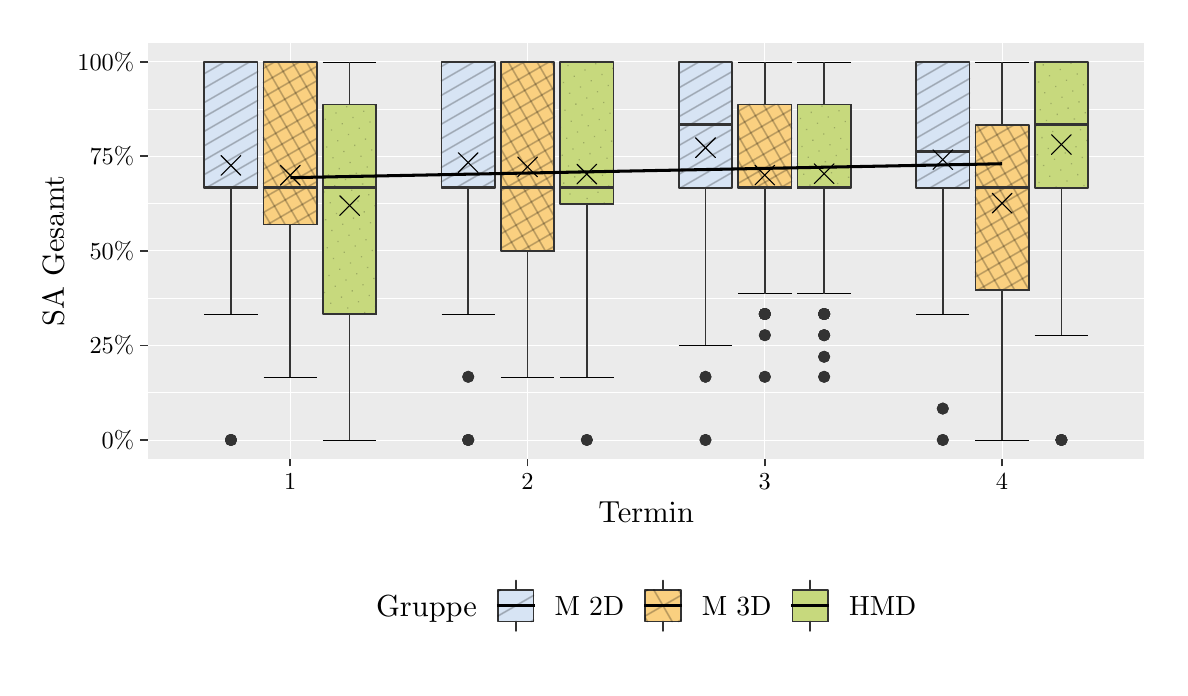
\begin{tikzpicture}[x=1pt,y=1pt]
\definecolor{fillColor}{RGB}{255,255,255}
\path[use as bounding box,fill=fillColor,fill opacity=0.00] (0,0) rectangle (409.05,231.26);
\begin{scope}
\path[clip] (  0.00,  0.00) rectangle (409.05,231.26);
\definecolor{drawColor}{RGB}{255,255,255}
\definecolor{fillColor}{RGB}{255,255,255}

\path[draw=drawColor,line width= 0.6pt,line join=round,line cap=round,fill=fillColor] (  0.00, -0.00) rectangle (409.05,231.26);
\end{scope}
\begin{scope}
\path[clip] ( 43.44, 75.45) rectangle (403.55,225.76);
\definecolor{fillColor}{gray}{0.92}

\path[fill=fillColor] ( 43.44, 75.45) rectangle (403.55,225.76);
\definecolor{drawColor}{RGB}{255,255,255}

\path[draw=drawColor,line width= 0.3pt,line join=round] ( 43.44, 99.36) --
	(403.55, 99.36);

\path[draw=drawColor,line width= 0.3pt,line join=round] ( 43.44,133.52) --
	(403.55,133.52);

\path[draw=drawColor,line width= 0.3pt,line join=round] ( 43.44,167.69) --
	(403.55,167.69);

\path[draw=drawColor,line width= 0.3pt,line join=round] ( 43.44,201.85) --
	(403.55,201.85);

\path[draw=drawColor,line width= 0.3pt,line join=round] ( 43.44, 82.28) --
	(403.55, 82.28);

\path[draw=drawColor,line width= 0.3pt,line join=round] ( 43.44,116.44) --
	(403.55,116.44);

\path[draw=drawColor,line width= 0.3pt,line join=round] ( 43.44,150.61) --
	(403.55,150.61);

\path[draw=drawColor,line width= 0.3pt,line join=round] ( 43.44,184.77) --
	(403.55,184.77);

\path[draw=drawColor,line width= 0.3pt,line join=round] ( 43.44,218.93) --
	(403.55,218.93);

\path[draw=drawColor,line width= 0.3pt,line join=round] ( 94.89, 75.45) --
	( 94.89,225.76);

\path[draw=drawColor,line width= 0.3pt,line join=round] (180.63, 75.45) --
	(180.63,225.76);

\path[draw=drawColor,line width= 0.3pt,line join=round] (266.37, 75.45) --
	(266.37,225.76);

\path[draw=drawColor,line width= 0.3pt,line join=round] (352.10, 75.45) --
	(352.10,225.76);
\definecolor{drawColor}{RGB}{0,0,0}

\path[draw=drawColor,line width= 0.2pt,line join=round] ( 63.81,218.93) --
	( 83.10,218.93);

\path[draw=drawColor,line width= 0.2pt,line join=round] ( 73.45,218.93) --
	( 73.45,127.79);

\path[draw=drawColor,line width= 0.2pt,line join=round] ( 63.81,127.79) --
	( 83.10,127.79);

\path[draw=drawColor,line width= 0.2pt,line join=round] ( 85.24,218.93) --
	(104.53,218.93);

\path[draw=drawColor,line width= 0.2pt,line join=round] ( 94.89,218.93) --
	( 94.89,105.10);

\path[draw=drawColor,line width= 0.2pt,line join=round] ( 85.24,105.10) --
	(104.53,105.10);

\path[draw=drawColor,line width= 0.2pt,line join=round] (106.68,218.93) --
	(125.97,218.93);

\path[draw=drawColor,line width= 0.2pt,line join=round] (116.32,218.93) --
	(116.32, 82.28);

\path[draw=drawColor,line width= 0.2pt,line join=round] (106.68, 82.28) --
	(125.97, 82.28);

\path[draw=drawColor,line width= 0.2pt,line join=round] (149.55,218.93) --
	(168.84,218.93);

\path[draw=drawColor,line width= 0.2pt,line join=round] (159.19,218.93) --
	(159.19,127.79);

\path[draw=drawColor,line width= 0.2pt,line join=round] (149.55,127.79) --
	(168.84,127.79);

\path[draw=drawColor,line width= 0.2pt,line join=round] (170.98,218.93) --
	(190.27,218.93);

\path[draw=drawColor,line width= 0.2pt,line join=round] (180.63,218.93) --
	(180.63,105.10);

\path[draw=drawColor,line width= 0.2pt,line join=round] (170.98,105.10) --
	(190.27,105.10);

\path[draw=drawColor,line width= 0.2pt,line join=round] (192.41,218.93) --
	(211.71,218.93);

\path[draw=drawColor,line width= 0.2pt,line join=round] (202.06,218.93) --
	(202.06,105.10);

\path[draw=drawColor,line width= 0.2pt,line join=round] (192.41,105.10) --
	(211.71,105.10);

\path[draw=drawColor,line width= 0.2pt,line join=round] (235.28,218.93) --
	(254.58,218.93);

\path[draw=drawColor,line width= 0.2pt,line join=round] (244.93,218.93) --
	(244.93,116.44);

\path[draw=drawColor,line width= 0.2pt,line join=round] (235.28,116.44) --
	(254.58,116.44);

\path[draw=drawColor,line width= 0.2pt,line join=round] (256.72,218.93) --
	(276.01,218.93);

\path[draw=drawColor,line width= 0.2pt,line join=round] (266.37,218.93) --
	(266.37,135.16);

\path[draw=drawColor,line width= 0.2pt,line join=round] (256.72,135.16) --
	(276.01,135.16);

\path[draw=drawColor,line width= 0.2pt,line join=round] (278.15,218.93) --
	(297.45,218.93);

\path[draw=drawColor,line width= 0.2pt,line join=round] (287.80,218.93) --
	(287.80,135.16);

\path[draw=drawColor,line width= 0.2pt,line join=round] (278.15,135.16) --
	(297.45,135.16);

\path[draw=drawColor,line width= 0.2pt,line join=round] (321.02,218.93) --
	(340.32,218.93);

\path[draw=drawColor,line width= 0.2pt,line join=round] (330.67,218.93) --
	(330.67,127.79);

\path[draw=drawColor,line width= 0.2pt,line join=round] (321.02,127.79) --
	(340.32,127.79);

\path[draw=drawColor,line width= 0.2pt,line join=round] (342.46,218.93) --
	(361.75,218.93);

\path[draw=drawColor,line width= 0.2pt,line join=round] (352.10,218.93) --
	(352.10, 82.28);

\path[draw=drawColor,line width= 0.2pt,line join=round] (342.46, 82.28) --
	(361.75, 82.28);

\path[draw=drawColor,line width= 0.2pt,line join=round] (363.89,218.93) --
	(383.19,218.93);

\path[draw=drawColor,line width= 0.2pt,line join=round] (373.54,218.93) --
	(373.54,120.13);

\path[draw=drawColor,line width= 0.2pt,line join=round] (363.89,120.13) --
	(383.19,120.13);
\definecolor{drawColor}{gray}{0.20}
\definecolor{fillColor}{gray}{0.20}

\path[draw=drawColor,line width= 0.4pt,line join=round,line cap=round,fill=fillColor] ( 73.45, 82.28) circle (  1.96);

\path[draw=drawColor,line width= 0.4pt,line join=round,line cap=round,fill=fillColor] ( 73.45, 82.28) circle (  1.96);

\path[draw=drawColor,line width= 0.2pt,line join=round] ( 73.45,218.93) -- ( 73.45,218.93);

\path[draw=drawColor,line width= 0.2pt,line join=round] ( 73.45,173.43) -- ( 73.45,127.79);
\definecolor{fillColor}{RGB}{215,228,244}

\path[draw=drawColor,line width= 0.2pt,fill=fillColor] ( 63.81,218.93) --
	( 63.81,173.43) --
	( 83.10,173.43) --
	( 83.10,218.93) --
	( 63.81,218.93) --
	cycle;

\path[draw=drawColor,line width= 0.5pt] ( 63.81,173.43) -- ( 83.10,173.43);

\path[draw=drawColor,line width= 0.2pt,line join=round] ( 94.89,218.93) -- ( 94.89,218.93);

\path[draw=drawColor,line width= 0.2pt,line join=round] ( 94.89,160.17) -- ( 94.89,105.10);
\definecolor{fillColor}{RGB}{250,208,128}

\path[draw=drawColor,line width= 0.2pt,fill=fillColor] ( 85.24,218.93) --
	( 85.24,160.17) --
	(104.53,160.17) --
	(104.53,218.93) --
	( 85.24,218.93) --
	cycle;

\path[draw=drawColor,line width= 0.5pt] ( 85.24,173.43) -- (104.53,173.43);

\path[draw=drawColor,line width= 0.2pt,line join=round] (116.32,203.49) -- (116.32,218.93);

\path[draw=drawColor,line width= 0.2pt,line join=round] (116.32,127.79) -- (116.32, 82.28);
\definecolor{fillColor}{RGB}{199,217,125}

\path[draw=drawColor,line width= 0.2pt,fill=fillColor] (106.68,203.49) --
	(106.68,127.79) --
	(125.97,127.79) --
	(125.97,203.49) --
	(106.68,203.49) --
	cycle;

\path[draw=drawColor,line width= 0.5pt] (106.68,173.43) -- (125.97,173.43);
\definecolor{fillColor}{gray}{0.20}

\path[draw=drawColor,line width= 0.4pt,line join=round,line cap=round,fill=fillColor] (159.19, 82.28) circle (  1.96);

\path[draw=drawColor,line width= 0.4pt,line join=round,line cap=round,fill=fillColor] (159.19,105.10) circle (  1.96);

\path[draw=drawColor,line width= 0.4pt,line join=round,line cap=round,fill=fillColor] (159.19, 82.28) circle (  1.96);

\path[draw=drawColor,line width= 0.2pt,line join=round] (159.19,218.93) -- (159.19,218.93);

\path[draw=drawColor,line width= 0.2pt,line join=round] (159.19,173.43) -- (159.19,127.79);
\definecolor{fillColor}{RGB}{215,228,244}

\path[draw=drawColor,line width= 0.2pt,fill=fillColor] (149.55,218.93) --
	(149.55,173.43) --
	(168.84,173.43) --
	(168.84,218.93) --
	(149.55,218.93) --
	cycle;

\path[draw=drawColor,line width= 0.5pt] (149.55,173.43) -- (168.84,173.43);

\path[draw=drawColor,line width= 0.2pt,line join=round] (180.63,218.93) -- (180.63,218.93);

\path[draw=drawColor,line width= 0.2pt,line join=round] (180.63,150.61) -- (180.63,105.10);
\definecolor{fillColor}{RGB}{250,208,128}

\path[draw=drawColor,line width= 0.2pt,fill=fillColor] (170.98,218.93) --
	(170.98,150.61) --
	(190.27,150.61) --
	(190.27,218.93) --
	(170.98,218.93) --
	cycle;

\path[draw=drawColor,line width= 0.5pt] (170.98,173.43) -- (190.27,173.43);
\definecolor{fillColor}{gray}{0.20}

\path[draw=drawColor,line width= 0.4pt,line join=round,line cap=round,fill=fillColor] (202.06, 82.28) circle (  1.96);

\path[draw=drawColor,line width= 0.2pt,line join=round] (202.06,218.93) -- (202.06,218.93);

\path[draw=drawColor,line width= 0.2pt,line join=round] (202.06,167.58) -- (202.06,105.10);
\definecolor{fillColor}{RGB}{199,217,125}

\path[draw=drawColor,line width= 0.2pt,fill=fillColor] (192.41,218.93) --
	(192.41,167.58) --
	(211.71,167.58) --
	(211.71,218.93) --
	(192.41,218.93) --
	cycle;

\path[draw=drawColor,line width= 0.5pt] (192.41,173.43) -- (211.71,173.43);
\definecolor{fillColor}{gray}{0.20}

\path[draw=drawColor,line width= 0.4pt,line join=round,line cap=round,fill=fillColor] (244.93, 82.28) circle (  1.96);

\path[draw=drawColor,line width= 0.4pt,line join=round,line cap=round,fill=fillColor] (244.93,105.10) circle (  1.96);

\path[draw=drawColor,line width= 0.2pt,line join=round] (244.93,218.93) -- (244.93,218.93);

\path[draw=drawColor,line width= 0.2pt,line join=round] (244.93,173.43) -- (244.93,116.44);
\definecolor{fillColor}{RGB}{215,228,244}

\path[draw=drawColor,line width= 0.2pt,fill=fillColor] (235.28,218.93) --
	(235.28,173.43) --
	(254.58,173.43) --
	(254.58,218.93) --
	(235.28,218.93) --
	cycle;

\path[draw=drawColor,line width= 0.5pt] (235.28,196.11) -- (254.58,196.11);
\definecolor{fillColor}{gray}{0.20}

\path[draw=drawColor,line width= 0.4pt,line join=round,line cap=round,fill=fillColor] (266.37,127.79) circle (  1.96);

\path[draw=drawColor,line width= 0.4pt,line join=round,line cap=round,fill=fillColor] (266.37,127.79) circle (  1.96);

\path[draw=drawColor,line width= 0.4pt,line join=round,line cap=round,fill=fillColor] (266.37,127.79) circle (  1.96);

\path[draw=drawColor,line width= 0.4pt,line join=round,line cap=round,fill=fillColor] (266.37,127.79) circle (  1.96);

\path[draw=drawColor,line width= 0.4pt,line join=round,line cap=round,fill=fillColor] (266.37,120.13) circle (  1.96);

\path[draw=drawColor,line width= 0.4pt,line join=round,line cap=round,fill=fillColor] (266.37,105.10) circle (  1.96);

\path[draw=drawColor,line width= 0.4pt,line join=round,line cap=round,fill=fillColor] (266.37,127.79) circle (  1.96);

\path[draw=drawColor,line width= 0.2pt,line join=round] (266.37,203.49) -- (266.37,218.93);

\path[draw=drawColor,line width= 0.2pt,line join=round] (266.37,173.43) -- (266.37,135.16);
\definecolor{fillColor}{RGB}{250,208,128}

\path[draw=drawColor,line width= 0.2pt,fill=fillColor] (256.72,203.49) --
	(256.72,173.43) --
	(276.01,173.43) --
	(276.01,203.49) --
	(256.72,203.49) --
	cycle;

\path[draw=drawColor,line width= 0.5pt] (256.72,173.43) -- (276.01,173.43);
\definecolor{fillColor}{gray}{0.20}

\path[draw=drawColor,line width= 0.4pt,line join=round,line cap=round,fill=fillColor] (287.80,127.79) circle (  1.96);

\path[draw=drawColor,line width= 0.4pt,line join=round,line cap=round,fill=fillColor] (287.80,127.79) circle (  1.96);

\path[draw=drawColor,line width= 0.4pt,line join=round,line cap=round,fill=fillColor] (287.80,127.79) circle (  1.96);

\path[draw=drawColor,line width= 0.4pt,line join=round,line cap=round,fill=fillColor] (287.80,120.13) circle (  1.96);

\path[draw=drawColor,line width= 0.4pt,line join=round,line cap=round,fill=fillColor] (287.80,112.34) circle (  1.96);

\path[draw=drawColor,line width= 0.4pt,line join=round,line cap=round,fill=fillColor] (287.80,127.79) circle (  1.96);

\path[draw=drawColor,line width= 0.4pt,line join=round,line cap=round,fill=fillColor] (287.80,120.13) circle (  1.96);

\path[draw=drawColor,line width= 0.4pt,line join=round,line cap=round,fill=fillColor] (287.80,105.10) circle (  1.96);

\path[draw=drawColor,line width= 0.4pt,line join=round,line cap=round,fill=fillColor] (287.80,127.79) circle (  1.96);

\path[draw=drawColor,line width= 0.2pt,line join=round] (287.80,203.49) -- (287.80,218.93);

\path[draw=drawColor,line width= 0.2pt,line join=round] (287.80,173.43) -- (287.80,135.16);
\definecolor{fillColor}{RGB}{199,217,125}

\path[draw=drawColor,line width= 0.2pt,fill=fillColor] (278.15,203.49) --
	(278.15,173.43) --
	(297.45,173.43) --
	(297.45,203.49) --
	(278.15,203.49) --
	cycle;

\path[draw=drawColor,line width= 0.5pt] (278.15,173.43) -- (297.45,173.43);
\definecolor{fillColor}{gray}{0.20}

\path[draw=drawColor,line width= 0.4pt,line join=round,line cap=round,fill=fillColor] (330.67, 82.28) circle (  1.96);

\path[draw=drawColor,line width= 0.4pt,line join=round,line cap=round,fill=fillColor] (330.67, 93.62) circle (  1.96);

\path[draw=drawColor,line width= 0.2pt,line join=round] (330.67,218.93) -- (330.67,218.93);

\path[draw=drawColor,line width= 0.2pt,line join=round] (330.67,173.43) -- (330.67,127.79);
\definecolor{fillColor}{RGB}{215,228,244}

\path[draw=drawColor,line width= 0.2pt,fill=fillColor] (321.02,218.93) --
	(321.02,173.43) --
	(340.32,173.43) --
	(340.32,218.93) --
	(321.02,218.93) --
	cycle;

\path[draw=drawColor,line width= 0.5pt] (321.02,186.55) -- (340.32,186.55);

\path[draw=drawColor,line width= 0.2pt,line join=round] (352.10,196.11) -- (352.10,218.93);

\path[draw=drawColor,line width= 0.2pt,line join=round] (352.10,136.39) -- (352.10, 82.28);
\definecolor{fillColor}{RGB}{250,208,128}

\path[draw=drawColor,line width= 0.2pt,fill=fillColor] (342.46,196.11) --
	(342.46,136.39) --
	(361.75,136.39) --
	(361.75,196.11) --
	(342.46,196.11) --
	cycle;

\path[draw=drawColor,line width= 0.5pt] (342.46,173.43) -- (361.75,173.43);
\definecolor{fillColor}{gray}{0.20}

\path[draw=drawColor,line width= 0.4pt,line join=round,line cap=round,fill=fillColor] (373.54, 82.28) circle (  1.96);

\path[draw=drawColor,line width= 0.4pt,line join=round,line cap=round,fill=fillColor] (373.54, 82.28) circle (  1.96);

\path[draw=drawColor,line width= 0.2pt,line join=round] (373.54,218.93) -- (373.54,218.93);

\path[draw=drawColor,line width= 0.2pt,line join=round] (373.54,173.43) -- (373.54,120.13);
\definecolor{fillColor}{RGB}{199,217,125}

\path[draw=drawColor,line width= 0.2pt,fill=fillColor] (363.89,218.93) --
	(363.89,173.43) --
	(383.19,173.43) --
	(383.19,218.93) --
	(363.89,218.93) --
	cycle;

\path[draw=drawColor,line width= 0.5pt] (363.89,196.11) -- (383.19,196.11);
\definecolor{fillColor}{gray}{0.20}

\path[draw=drawColor,line width= 0.4pt,line join=round,line cap=round,fill=fillColor] ( 73.45, 82.28) circle (  1.96);

\path[draw=drawColor,line width= 0.4pt,line join=round,line cap=round,fill=fillColor] ( 73.45, 82.28) circle (  1.96);

\path[draw=drawColor,line width= 0.6pt,line join=round] ( 73.45,218.93) -- ( 73.45,218.93);

\path[draw=drawColor,line width= 0.6pt,line join=round] ( 73.45,173.43) -- ( 73.45,127.79);
\definecolor{fillColor}{RGB}{215,228,244}

\path[fill=fillColor] ( 63.81,218.93) --
	( 63.81,173.43) --
	( 83.10,173.43) --
	( 83.10,218.93) --
	( 63.81,218.93) --
	cycle;
\definecolor{drawColor}{RGB}{0,0,0}
\definecolor{fillColor}{RGB}{0,0,0}

\path[draw=drawColor,draw opacity=0.20,line width= 0.6pt,line join=round,line cap=rect,fill=fillColor,fill opacity=0.20] ( 83.10,173.72) --
	( 83.10,173.66) --
	( 82.69,173.43) --
	( 82.60,173.43) --
	( 83.10,173.72) --
	cycle;

\path[draw=drawColor,draw opacity=0.20,line width= 0.6pt,line join=round,line cap=rect,fill=fillColor,fill opacity=0.20] ( 83.10,178.92) --
	( 83.10,178.87) --
	( 73.67,173.43) --
	( 73.58,173.43) --
	( 83.10,178.92) --
	cycle;

\path[draw=drawColor,draw opacity=0.20,line width= 0.6pt,line join=round,line cap=rect,fill=fillColor,fill opacity=0.20] ( 83.10,184.13) --
	( 83.10,184.08) --
	( 64.65,173.43) --
	( 64.56,173.43) --
	( 83.10,184.13) --
	cycle;

\path[draw=drawColor,draw opacity=0.20,line width= 0.6pt,line join=round,line cap=rect,fill=fillColor,fill opacity=0.20] ( 83.10,189.34) --
	( 83.10,189.28) --
	( 63.81,178.15) --
	( 63.81,178.20) --
	( 83.10,189.34) --
	cycle;

\path[draw=drawColor,draw opacity=0.20,line width= 0.6pt,line join=round,line cap=rect,fill=fillColor,fill opacity=0.20] ( 83.10,194.54) --
	( 83.10,194.49) --
	( 63.81,183.35) --
	( 63.81,183.41) --
	( 83.10,194.54) --
	cycle;

\path[draw=drawColor,draw opacity=0.20,line width= 0.6pt,line join=round,line cap=rect,fill=fillColor,fill opacity=0.20] ( 83.10,199.75) --
	( 83.10,199.70) --
	( 63.81,188.56) --
	( 63.81,188.61) --
	( 83.10,199.75) --
	cycle;

\path[draw=drawColor,draw opacity=0.20,line width= 0.6pt,line join=round,line cap=rect,fill=fillColor,fill opacity=0.20] ( 83.10,204.96) --
	( 83.10,204.91) --
	( 63.81,193.77) --
	( 63.81,193.82) --
	( 83.10,204.96) --
	cycle;

\path[draw=drawColor,draw opacity=0.20,line width= 0.6pt,line join=round,line cap=rect,fill=fillColor,fill opacity=0.20] ( 83.10,210.16) --
	( 83.10,210.11) --
	( 63.81,198.97) --
	( 63.81,199.03) --
	( 83.10,210.16) --
	cycle;

\path[draw=drawColor,draw opacity=0.20,line width= 0.6pt,line join=round,line cap=rect,fill=fillColor,fill opacity=0.20] ( 83.10,215.37) --
	( 83.10,215.32) --
	( 63.81,204.18) --
	( 63.81,204.23) --
	( 83.10,215.37) --
	cycle;

\path[draw=drawColor,draw opacity=0.20,line width= 0.6pt,line join=round,line cap=rect,fill=fillColor,fill opacity=0.20] ( 80.24,218.93) --
	( 80.33,218.93) --
	( 63.81,209.39) --
	( 63.81,209.44) --
	( 80.24,218.93) --
	cycle;

\path[draw=drawColor,draw opacity=0.20,line width= 0.6pt,line join=round,line cap=rect,fill=fillColor,fill opacity=0.20] ( 71.22,218.93) --
	( 71.31,218.93) --
	( 63.81,214.60) --
	( 63.81,214.65) --
	( 71.22,218.93) --
	cycle;
\definecolor{drawColor}{gray}{0.20}

\path[draw=drawColor,line width= 0.6pt,line join=round,line cap=round] ( 63.81,218.93) --
	( 63.81,173.43) --
	( 83.10,173.43) --
	( 83.10,218.93) --
	( 63.81,218.93) --
	cycle;

\path[draw=drawColor,line width= 1.1pt,line join=round] ( 63.81,173.43) -- ( 83.10,173.43);
\definecolor{fillColor}{gray}{0.20}

\path[draw=drawColor,line width= 0.4pt,line join=round,line cap=round,fill=fillColor] (159.19, 82.28) circle (  1.96);

\path[draw=drawColor,line width= 0.4pt,line join=round,line cap=round,fill=fillColor] (159.19,105.10) circle (  1.96);

\path[draw=drawColor,line width= 0.4pt,line join=round,line cap=round,fill=fillColor] (159.19, 82.28) circle (  1.96);

\path[draw=drawColor,line width= 0.6pt,line join=round] (159.19,218.93) -- (159.19,218.93);

\path[draw=drawColor,line width= 0.6pt,line join=round] (159.19,173.43) -- (159.19,127.79);
\definecolor{fillColor}{RGB}{215,228,244}

\path[fill=fillColor] (149.55,218.93) --
	(149.55,173.43) --
	(168.84,173.43) --
	(168.84,218.93) --
	(149.55,218.93) --
	cycle;
\definecolor{drawColor}{RGB}{0,0,0}
\definecolor{fillColor}{RGB}{0,0,0}

\path[draw=drawColor,draw opacity=0.20,line width= 0.6pt,line join=round,line cap=rect,fill=fillColor,fill opacity=0.20] (168.84,176.35) --
	(168.84,176.30) --
	(163.86,173.43) --
	(163.77,173.43) --
	(168.84,176.35) --
	cycle;

\path[draw=drawColor,draw opacity=0.20,line width= 0.6pt,line join=round,line cap=rect,fill=fillColor,fill opacity=0.20] (168.84,181.56) --
	(168.84,181.51) --
	(154.84,173.43) --
	(154.75,173.43) --
	(168.84,181.56) --
	cycle;

\path[draw=drawColor,draw opacity=0.20,line width= 0.6pt,line join=round,line cap=rect,fill=fillColor,fill opacity=0.20] (168.84,186.77) --
	(168.84,186.71) --
	(149.55,175.58) --
	(149.55,175.63) --
	(168.84,186.77) --
	cycle;

\path[draw=drawColor,draw opacity=0.20,line width= 0.6pt,line join=round,line cap=rect,fill=fillColor,fill opacity=0.20] (168.84,191.97) --
	(168.84,191.92) --
	(149.55,180.78) --
	(149.55,180.84) --
	(168.84,191.97) --
	cycle;

\path[draw=drawColor,draw opacity=0.20,line width= 0.6pt,line join=round,line cap=rect,fill=fillColor,fill opacity=0.20] (168.84,197.18) --
	(168.84,197.13) --
	(149.55,185.99) --
	(149.55,186.04) --
	(168.84,197.18) --
	cycle;

\path[draw=drawColor,draw opacity=0.20,line width= 0.6pt,line join=round,line cap=rect,fill=fillColor,fill opacity=0.20] (168.84,202.39) --
	(168.84,202.34) --
	(149.55,191.20) --
	(149.55,191.25) --
	(168.84,202.39) --
	cycle;

\path[draw=drawColor,draw opacity=0.20,line width= 0.6pt,line join=round,line cap=rect,fill=fillColor,fill opacity=0.20] (168.84,207.60) --
	(168.84,207.54) --
	(149.55,196.41) --
	(149.55,196.46) --
	(168.84,207.60) --
	cycle;

\path[draw=drawColor,draw opacity=0.20,line width= 0.6pt,line join=round,line cap=rect,fill=fillColor,fill opacity=0.20] (168.84,212.80) --
	(168.84,212.75) --
	(149.55,201.61) --
	(149.55,201.66) --
	(168.84,212.80) --
	cycle;

\path[draw=drawColor,draw opacity=0.20,line width= 0.6pt,line join=round,line cap=rect,fill=fillColor,fill opacity=0.20] (168.84,218.01) --
	(168.84,217.96) --
	(149.55,206.82) --
	(149.55,206.87) --
	(168.84,218.01) --
	cycle;

\path[draw=drawColor,draw opacity=0.20,line width= 0.6pt,line join=round,line cap=rect,fill=fillColor,fill opacity=0.20] (161.41,218.93) --
	(161.50,218.93) --
	(149.55,212.03) --
	(149.55,212.08) --
	(161.41,218.93) --
	cycle;

\path[draw=drawColor,draw opacity=0.20,line width= 0.6pt,line join=round,line cap=rect,fill=fillColor,fill opacity=0.20] (152.40,218.93) --
	(152.49,218.93) --
	(149.55,217.23) --
	(149.55,217.29) --
	(152.40,218.93) --
	cycle;
\definecolor{drawColor}{gray}{0.20}

\path[draw=drawColor,line width= 0.6pt,line join=round,line cap=round] (149.55,218.93) --
	(149.55,173.43) --
	(168.84,173.43) --
	(168.84,218.93) --
	(149.55,218.93) --
	cycle;

\path[draw=drawColor,line width= 1.1pt,line join=round] (149.55,173.43) -- (168.84,173.43);
\definecolor{fillColor}{gray}{0.20}

\path[draw=drawColor,line width= 0.4pt,line join=round,line cap=round,fill=fillColor] (244.93, 82.28) circle (  1.96);

\path[draw=drawColor,line width= 0.4pt,line join=round,line cap=round,fill=fillColor] (244.93,105.10) circle (  1.96);

\path[draw=drawColor,line width= 0.6pt,line join=round] (244.93,218.93) -- (244.93,218.93);

\path[draw=drawColor,line width= 0.6pt,line join=round] (244.93,173.43) -- (244.93,116.44);
\definecolor{fillColor}{RGB}{215,228,244}

\path[fill=fillColor] (235.28,218.93) --
	(235.28,173.43) --
	(254.58,173.43) --
	(254.58,218.93) --
	(235.28,218.93) --
	cycle;
\definecolor{drawColor}{RGB}{0,0,0}
\definecolor{fillColor}{RGB}{0,0,0}

\path[draw=drawColor,draw opacity=0.20,line width= 0.6pt,line join=round,line cap=rect,fill=fillColor,fill opacity=0.20] (254.58,173.78) --
	(254.58,173.73) --
	(254.05,173.43) --
	(253.96,173.43) --
	(254.58,173.78) --
	cycle;

\path[draw=drawColor,draw opacity=0.20,line width= 0.6pt,line join=round,line cap=rect,fill=fillColor,fill opacity=0.20] (254.58,178.99) --
	(254.58,178.94) --
	(245.03,173.43) --
	(244.94,173.43) --
	(254.58,178.99) --
	cycle;

\path[draw=drawColor,draw opacity=0.20,line width= 0.6pt,line join=round,line cap=rect,fill=fillColor,fill opacity=0.20] (254.58,184.20) --
	(254.58,184.15) --
	(236.01,173.43) --
	(235.92,173.43) --
	(254.58,184.20) --
	cycle;

\path[draw=drawColor,draw opacity=0.20,line width= 0.6pt,line join=round,line cap=rect,fill=fillColor,fill opacity=0.20] (254.58,189.40) --
	(254.58,189.35) --
	(235.28,178.21) --
	(235.28,178.27) --
	(254.58,189.40) --
	cycle;

\path[draw=drawColor,draw opacity=0.20,line width= 0.6pt,line join=round,line cap=rect,fill=fillColor,fill opacity=0.20] (254.58,194.61) --
	(254.58,194.56) --
	(235.28,183.42) --
	(235.28,183.47) --
	(254.58,194.61) --
	cycle;

\path[draw=drawColor,draw opacity=0.20,line width= 0.6pt,line join=round,line cap=rect,fill=fillColor,fill opacity=0.20] (254.58,199.82) --
	(254.58,199.77) --
	(235.28,188.63) --
	(235.28,188.68) --
	(254.58,199.82) --
	cycle;

\path[draw=drawColor,draw opacity=0.20,line width= 0.6pt,line join=round,line cap=rect,fill=fillColor,fill opacity=0.20] (254.58,205.03) --
	(254.58,204.97) --
	(235.28,193.84) --
	(235.28,193.89) --
	(254.58,205.03) --
	cycle;

\path[draw=drawColor,draw opacity=0.20,line width= 0.6pt,line join=round,line cap=rect,fill=fillColor,fill opacity=0.20] (254.58,210.23) --
	(254.58,210.18) --
	(235.28,199.04) --
	(235.28,199.10) --
	(254.58,210.23) --
	cycle;

\path[draw=drawColor,draw opacity=0.20,line width= 0.6pt,line join=round,line cap=rect,fill=fillColor,fill opacity=0.20] (254.58,215.44) --
	(254.58,215.39) --
	(235.28,204.25) --
	(235.28,204.30) --
	(254.58,215.44) --
	cycle;

\path[draw=drawColor,draw opacity=0.20,line width= 0.6pt,line join=round,line cap=rect,fill=fillColor,fill opacity=0.20] (251.60,218.93) --
	(251.69,218.93) --
	(235.28,209.46) --
	(235.28,209.51) --
	(251.60,218.93) --
	cycle;

\path[draw=drawColor,draw opacity=0.20,line width= 0.6pt,line join=round,line cap=rect,fill=fillColor,fill opacity=0.20] (242.58,218.93) --
	(242.68,218.93) --
	(235.28,214.66) --
	(235.28,214.72) --
	(242.58,218.93) --
	cycle;
\definecolor{drawColor}{gray}{0.20}

\path[draw=drawColor,line width= 0.6pt,line join=round,line cap=round] (235.28,218.93) --
	(235.28,173.43) --
	(254.58,173.43) --
	(254.58,218.93) --
	(235.28,218.93) --
	cycle;

\path[draw=drawColor,line width= 1.1pt,line join=round] (235.28,196.11) -- (254.58,196.11);
\definecolor{fillColor}{gray}{0.20}

\path[draw=drawColor,line width= 0.4pt,line join=round,line cap=round,fill=fillColor] (330.67, 82.28) circle (  1.96);

\path[draw=drawColor,line width= 0.4pt,line join=round,line cap=round,fill=fillColor] (330.67, 93.62) circle (  1.96);

\path[draw=drawColor,line width= 0.6pt,line join=round] (330.67,218.93) -- (330.67,218.93);

\path[draw=drawColor,line width= 0.6pt,line join=round] (330.67,173.43) -- (330.67,127.79);
\definecolor{fillColor}{RGB}{215,228,244}

\path[fill=fillColor] (321.02,218.93) --
	(321.02,173.43) --
	(340.32,173.43) --
	(340.32,218.93) --
	(321.02,218.93) --
	cycle;
\definecolor{drawColor}{RGB}{0,0,0}
\definecolor{fillColor}{RGB}{0,0,0}

\path[draw=drawColor,draw opacity=0.20,line width= 0.6pt,line join=round,line cap=rect,fill=fillColor,fill opacity=0.20] (340.32,176.42) --
	(340.32,176.37) --
	(335.22,173.43) --
	(335.13,173.43) --
	(340.32,176.42) --
	cycle;

\path[draw=drawColor,draw opacity=0.20,line width= 0.6pt,line join=round,line cap=rect,fill=fillColor,fill opacity=0.20] (340.32,181.63) --
	(340.32,181.58) --
	(326.20,173.43) --
	(326.11,173.43) --
	(340.32,181.63) --
	cycle;

\path[draw=drawColor,draw opacity=0.20,line width= 0.6pt,line join=round,line cap=rect,fill=fillColor,fill opacity=0.20] (340.32,186.84) --
	(340.32,186.78) --
	(321.02,175.65) --
	(321.02,175.70) --
	(340.32,186.84) --
	cycle;

\path[draw=drawColor,draw opacity=0.20,line width= 0.6pt,line join=round,line cap=rect,fill=fillColor,fill opacity=0.20] (340.32,192.04) --
	(340.32,191.99) --
	(321.02,180.85) --
	(321.02,180.90) --
	(340.32,192.04) --
	cycle;

\path[draw=drawColor,draw opacity=0.20,line width= 0.6pt,line join=round,line cap=rect,fill=fillColor,fill opacity=0.20] (340.32,197.25) --
	(340.32,197.20) --
	(321.02,186.06) --
	(321.02,186.11) --
	(340.32,197.25) --
	cycle;

\path[draw=drawColor,draw opacity=0.20,line width= 0.6pt,line join=round,line cap=rect,fill=fillColor,fill opacity=0.20] (340.32,202.46) --
	(340.32,202.40) --
	(321.02,191.27) --
	(321.02,191.32) --
	(340.32,202.46) --
	cycle;

\path[draw=drawColor,draw opacity=0.20,line width= 0.6pt,line join=round,line cap=rect,fill=fillColor,fill opacity=0.20] (340.32,207.66) --
	(340.32,207.61) --
	(321.02,196.47) --
	(321.02,196.53) --
	(340.32,207.66) --
	cycle;

\path[draw=drawColor,draw opacity=0.20,line width= 0.6pt,line join=round,line cap=rect,fill=fillColor,fill opacity=0.20] (340.32,212.87) --
	(340.32,212.82) --
	(321.02,201.68) --
	(321.02,201.73) --
	(340.32,212.87) --
	cycle;

\path[draw=drawColor,draw opacity=0.20,line width= 0.6pt,line join=round,line cap=rect,fill=fillColor,fill opacity=0.20] (340.32,218.08) --
	(340.32,218.03) --
	(321.02,206.89) --
	(321.02,206.94) --
	(340.32,218.08) --
	cycle;

\path[draw=drawColor,draw opacity=0.20,line width= 0.6pt,line join=round,line cap=rect,fill=fillColor,fill opacity=0.20] (332.77,218.93) --
	(332.86,218.93) --
	(321.02,212.10) --
	(321.02,212.15) --
	(332.77,218.93) --
	cycle;

\path[draw=drawColor,draw opacity=0.20,line width= 0.6pt,line join=round,line cap=rect,fill=fillColor,fill opacity=0.20] (323.76,218.93) --
	(323.85,218.93) --
	(321.02,217.30) --
	(321.02,217.35) --
	(323.76,218.93) --
	cycle;
\definecolor{drawColor}{gray}{0.20}

\path[draw=drawColor,line width= 0.6pt,line join=round,line cap=round] (321.02,218.93) --
	(321.02,173.43) --
	(340.32,173.43) --
	(340.32,218.93) --
	(321.02,218.93) --
	cycle;

\path[draw=drawColor,line width= 1.1pt,line join=round] (321.02,186.55) -- (340.32,186.55);

\path[draw=drawColor,line width= 0.6pt,line join=round] ( 94.89,218.93) -- ( 94.89,218.93);

\path[draw=drawColor,line width= 0.6pt,line join=round] ( 94.89,160.17) -- ( 94.89,105.10);
\definecolor{fillColor}{RGB}{250,208,128}

\path[fill=fillColor] ( 85.24,218.93) --
	( 85.24,160.17) --
	(104.53,160.17) --
	(104.53,218.93) --
	( 85.24,218.93) --
	cycle;
\definecolor{drawColor}{RGB}{0,0,0}
\definecolor{fillColor}{RGB}{0,0,0}

\path[draw=drawColor,draw opacity=0.20,line width= 0.6pt,line join=round,line cap=rect,fill=fillColor,fill opacity=0.20] (104.53,165.26) --
	(104.53,165.21) --
	( 95.81,160.17) --
	( 95.72,160.17) --
	(104.53,165.26) --
	cycle;

\path[draw=drawColor,draw opacity=0.20,line width= 0.6pt,line join=round,line cap=rect,fill=fillColor,fill opacity=0.20] (104.53,170.47) --
	(104.53,170.42) --
	( 86.79,160.17) --
	( 86.70,160.17) --
	(104.53,170.47) --
	cycle;

\path[draw=drawColor,draw opacity=0.20,line width= 0.6pt,line join=round,line cap=rect,fill=fillColor,fill opacity=0.20] (104.53,175.68) --
	(104.53,175.62) --
	( 85.24,164.49) --
	( 85.24,164.54) --
	(104.53,175.68) --
	cycle;

\path[draw=drawColor,draw opacity=0.20,line width= 0.6pt,line join=round,line cap=rect,fill=fillColor,fill opacity=0.20] (104.53,180.88) --
	(104.53,180.83) --
	( 85.24,169.69) --
	( 85.24,169.75) --
	(104.53,180.88) --
	cycle;

\path[draw=drawColor,draw opacity=0.20,line width= 0.6pt,line join=round,line cap=rect,fill=fillColor,fill opacity=0.20] (104.53,186.09) --
	(104.53,186.04) --
	( 85.24,174.90) --
	( 85.24,174.95) --
	(104.53,186.09) --
	cycle;

\path[draw=drawColor,draw opacity=0.20,line width= 0.6pt,line join=round,line cap=rect,fill=fillColor,fill opacity=0.20] (104.53,191.30) --
	(104.53,191.25) --
	( 85.24,180.11) --
	( 85.24,180.16) --
	(104.53,191.30) --
	cycle;

\path[draw=drawColor,draw opacity=0.20,line width= 0.6pt,line join=round,line cap=rect,fill=fillColor,fill opacity=0.20] (104.53,196.50) --
	(104.53,196.45) --
	( 85.24,185.31) --
	( 85.24,185.37) --
	(104.53,196.50) --
	cycle;

\path[draw=drawColor,draw opacity=0.20,line width= 0.6pt,line join=round,line cap=rect,fill=fillColor,fill opacity=0.20] (104.53,201.71) --
	(104.53,201.66) --
	( 85.24,190.52) --
	( 85.24,190.57) --
	(104.53,201.71) --
	cycle;

\path[draw=drawColor,draw opacity=0.20,line width= 0.6pt,line join=round,line cap=rect,fill=fillColor,fill opacity=0.20] (104.53,206.92) --
	(104.53,206.87) --
	( 85.24,195.73) --
	( 85.24,195.78) --
	(104.53,206.92) --
	cycle;

\path[draw=drawColor,draw opacity=0.20,line width= 0.6pt,line join=round,line cap=rect,fill=fillColor,fill opacity=0.20] (104.53,212.13) --
	(104.53,212.07) --
	( 85.24,200.94) --
	( 85.24,200.99) --
	(104.53,212.13) --
	cycle;

\path[draw=drawColor,draw opacity=0.20,line width= 0.6pt,line join=round,line cap=rect,fill=fillColor,fill opacity=0.20] (104.53,217.33) --
	(104.53,217.28) --
	( 85.24,206.14) --
	( 85.24,206.20) --
	(104.53,217.33) --
	cycle;

\path[draw=drawColor,draw opacity=0.20,line width= 0.6pt,line join=round,line cap=rect,fill=fillColor,fill opacity=0.20] ( 98.28,218.93) --
	( 98.37,218.93) --
	( 85.24,211.35) --
	( 85.24,211.40) --
	( 98.28,218.93) --
	cycle;

\path[draw=drawColor,draw opacity=0.20,line width= 0.6pt,line join=round,line cap=rect,fill=fillColor,fill opacity=0.20] ( 89.26,218.93) --
	( 89.35,218.93) --
	( 85.24,216.56) --
	( 85.24,216.61) --
	( 89.26,218.93) --
	cycle;

\path[draw=drawColor,draw opacity=0.20,line width= 0.6pt,line join=round,line cap=rect,fill=fillColor,fill opacity=0.20] ( 87.82,160.17) --
	( 87.77,160.17) --
	( 85.24,164.55) --
	( 85.24,164.64) --
	( 87.82,160.17) --
	cycle;

\path[draw=drawColor,draw opacity=0.20,line width= 0.6pt,line join=round,line cap=rect,fill=fillColor,fill opacity=0.20] ( 93.03,160.17) --
	( 92.98,160.17) --
	( 85.24,173.57) --
	( 85.24,173.66) --
	( 93.03,160.17) --
	cycle;

\path[draw=drawColor,draw opacity=0.20,line width= 0.6pt,line join=round,line cap=rect,fill=fillColor,fill opacity=0.20] ( 98.24,160.17) --
	( 98.18,160.17) --
	( 85.24,182.59) --
	( 85.24,182.68) --
	( 98.24,160.17) --
	cycle;

\path[draw=drawColor,draw opacity=0.20,line width= 0.6pt,line join=round,line cap=rect,fill=fillColor,fill opacity=0.20] (103.44,160.17) --
	(103.39,160.17) --
	( 85.24,191.61) --
	( 85.24,191.70) --
	(103.44,160.17) --
	cycle;

\path[draw=drawColor,draw opacity=0.20,line width= 0.6pt,line join=round,line cap=rect,fill=fillColor,fill opacity=0.20] (104.53,167.30) --
	(104.53,167.21) --
	( 85.24,200.63) --
	( 85.24,200.72) --
	(104.53,167.30) --
	cycle;

\path[draw=drawColor,draw opacity=0.20,line width= 0.6pt,line join=round,line cap=rect,fill=fillColor,fill opacity=0.20] (104.53,176.32) --
	(104.53,176.23) --
	( 85.24,209.65) --
	( 85.24,209.74) --
	(104.53,176.32) --
	cycle;

\path[draw=drawColor,draw opacity=0.20,line width= 0.6pt,line join=round,line cap=rect,fill=fillColor,fill opacity=0.20] (104.53,185.34) --
	(104.53,185.25) --
	( 85.24,218.66) --
	( 85.24,218.76) --
	(104.53,185.34) --
	cycle;

\path[draw=drawColor,draw opacity=0.20,line width= 0.6pt,line join=round,line cap=rect,fill=fillColor,fill opacity=0.20] (104.53,194.36) --
	(104.53,194.27) --
	( 90.29,218.93) --
	( 90.35,218.93) --
	(104.53,194.36) --
	cycle;

\path[draw=drawColor,draw opacity=0.20,line width= 0.6pt,line join=round,line cap=rect,fill=fillColor,fill opacity=0.20] (104.53,203.38) --
	(104.53,203.29) --
	( 95.50,218.93) --
	( 95.55,218.93) --
	(104.53,203.38) --
	cycle;

\path[draw=drawColor,draw opacity=0.20,line width= 0.6pt,line join=round,line cap=rect,fill=fillColor,fill opacity=0.20] (104.53,212.40) --
	(104.53,212.31) --
	(100.71,218.93) --
	(100.76,218.93) --
	(104.53,212.40) --
	cycle;
\definecolor{drawColor}{gray}{0.20}

\path[draw=drawColor,line width= 0.6pt,line join=round,line cap=round] ( 85.24,218.93) --
	( 85.24,160.17) --
	(104.53,160.17) --
	(104.53,218.93) --
	( 85.24,218.93) --
	cycle;

\path[draw=drawColor,line width= 1.1pt,line join=round] ( 85.24,173.43) -- (104.53,173.43);

\path[draw=drawColor,line width= 0.6pt,line join=round] (180.63,218.93) -- (180.63,218.93);

\path[draw=drawColor,line width= 0.6pt,line join=round] (180.63,150.61) -- (180.63,105.10);
\definecolor{fillColor}{RGB}{250,208,128}

\path[fill=fillColor] (170.98,218.93) --
	(170.98,150.61) --
	(190.27,150.61) --
	(190.27,218.93) --
	(170.98,218.93) --
	cycle;
\definecolor{drawColor}{RGB}{0,0,0}
\definecolor{fillColor}{RGB}{0,0,0}

\path[draw=drawColor,draw opacity=0.20,line width= 0.6pt,line join=round,line cap=rect,fill=fillColor,fill opacity=0.20] (190.27,152.28) --
	(190.27,152.23) --
	(187.46,150.61) --
	(187.37,150.61) --
	(190.27,152.28) --
	cycle;

\path[draw=drawColor,draw opacity=0.20,line width= 0.6pt,line join=round,line cap=rect,fill=fillColor,fill opacity=0.20] (190.27,157.49) --
	(190.27,157.43) --
	(178.45,150.61) --
	(178.36,150.61) --
	(190.27,157.49) --
	cycle;

\path[draw=drawColor,draw opacity=0.20,line width= 0.6pt,line join=round,line cap=rect,fill=fillColor,fill opacity=0.20] (190.27,162.69) --
	(190.27,162.64) --
	(170.98,151.50) --
	(170.98,151.55) --
	(190.27,162.69) --
	cycle;

\path[draw=drawColor,draw opacity=0.20,line width= 0.6pt,line join=round,line cap=rect,fill=fillColor,fill opacity=0.20] (190.27,167.90) --
	(190.27,167.85) --
	(170.98,156.71) --
	(170.98,156.76) --
	(190.27,167.90) --
	cycle;

\path[draw=drawColor,draw opacity=0.20,line width= 0.6pt,line join=round,line cap=rect,fill=fillColor,fill opacity=0.20] (190.27,173.11) --
	(190.27,173.05) --
	(170.98,161.92) --
	(170.98,161.97) --
	(190.27,173.11) --
	cycle;

\path[draw=drawColor,draw opacity=0.20,line width= 0.6pt,line join=round,line cap=rect,fill=fillColor,fill opacity=0.20] (190.27,178.31) --
	(190.27,178.26) --
	(170.98,167.12) --
	(170.98,167.18) --
	(190.27,178.31) --
	cycle;

\path[draw=drawColor,draw opacity=0.20,line width= 0.6pt,line join=round,line cap=rect,fill=fillColor,fill opacity=0.20] (190.27,183.52) --
	(190.27,183.47) --
	(170.98,172.33) --
	(170.98,172.38) --
	(190.27,183.52) --
	cycle;

\path[draw=drawColor,draw opacity=0.20,line width= 0.6pt,line join=round,line cap=rect,fill=fillColor,fill opacity=0.20] (190.27,188.73) --
	(190.27,188.68) --
	(170.98,177.54) --
	(170.98,177.59) --
	(190.27,188.73) --
	cycle;

\path[draw=drawColor,draw opacity=0.20,line width= 0.6pt,line join=round,line cap=rect,fill=fillColor,fill opacity=0.20] (190.27,193.94) --
	(190.27,193.88) --
	(170.98,182.75) --
	(170.98,182.80) --
	(190.27,193.94) --
	cycle;

\path[draw=drawColor,draw opacity=0.20,line width= 0.6pt,line join=round,line cap=rect,fill=fillColor,fill opacity=0.20] (190.27,199.14) --
	(190.27,199.09) --
	(170.98,187.95) --
	(170.98,188.00) --
	(190.27,199.14) --
	cycle;

\path[draw=drawColor,draw opacity=0.20,line width= 0.6pt,line join=round,line cap=rect,fill=fillColor,fill opacity=0.20] (190.27,204.35) --
	(190.27,204.30) --
	(170.98,193.16) --
	(170.98,193.21) --
	(190.27,204.35) --
	cycle;

\path[draw=drawColor,draw opacity=0.20,line width= 0.6pt,line join=round,line cap=rect,fill=fillColor,fill opacity=0.20] (190.27,209.56) --
	(190.27,209.50) --
	(170.98,198.37) --
	(170.98,198.42) --
	(190.27,209.56) --
	cycle;

\path[draw=drawColor,draw opacity=0.20,line width= 0.6pt,line join=round,line cap=rect,fill=fillColor,fill opacity=0.20] (190.27,214.76) --
	(190.27,214.71) --
	(170.98,203.57) --
	(170.98,203.63) --
	(190.27,214.76) --
	cycle;

\path[draw=drawColor,draw opacity=0.20,line width= 0.6pt,line join=round,line cap=rect,fill=fillColor,fill opacity=0.20] (188.47,218.93) --
	(188.56,218.93) --
	(170.98,208.78) --
	(170.98,208.83) --
	(188.47,218.93) --
	cycle;

\path[draw=drawColor,draw opacity=0.20,line width= 0.6pt,line join=round,line cap=rect,fill=fillColor,fill opacity=0.20] (179.45,218.93) --
	(179.54,218.93) --
	(170.98,213.99) --
	(170.98,214.04) --
	(179.45,218.93) --
	cycle;

\path[draw=drawColor,draw opacity=0.20,line width= 0.6pt,line join=round,line cap=rect,fill=fillColor,fill opacity=0.20] (171.45,150.61) --
	(171.40,150.61) --
	(170.98,151.33) --
	(170.98,151.42) --
	(171.45,150.61) --
	cycle;

\path[draw=drawColor,draw opacity=0.20,line width= 0.6pt,line join=round,line cap=rect,fill=fillColor,fill opacity=0.20] (176.66,150.61) --
	(176.61,150.61) --
	(170.98,160.35) --
	(170.98,160.44) --
	(176.66,150.61) --
	cycle;

\path[draw=drawColor,draw opacity=0.20,line width= 0.6pt,line join=round,line cap=rect,fill=fillColor,fill opacity=0.20] (181.86,150.61) --
	(181.81,150.61) --
	(170.98,169.37) --
	(170.98,169.46) --
	(181.86,150.61) --
	cycle;

\path[draw=drawColor,draw opacity=0.20,line width= 0.6pt,line join=round,line cap=rect,fill=fillColor,fill opacity=0.20] (187.07,150.61) --
	(187.02,150.61) --
	(170.98,178.39) --
	(170.98,178.48) --
	(187.07,150.61) --
	cycle;

\path[draw=drawColor,draw opacity=0.20,line width= 0.6pt,line join=round,line cap=rect,fill=fillColor,fill opacity=0.20] (190.27,154.08) --
	(190.27,153.99) --
	(170.98,187.41) --
	(170.98,187.50) --
	(190.27,154.08) --
	cycle;

\path[draw=drawColor,draw opacity=0.20,line width= 0.6pt,line join=round,line cap=rect,fill=fillColor,fill opacity=0.20] (190.27,163.10) --
	(190.27,163.01) --
	(170.98,196.43) --
	(170.98,196.52) --
	(190.27,163.10) --
	cycle;

\path[draw=drawColor,draw opacity=0.20,line width= 0.6pt,line join=round,line cap=rect,fill=fillColor,fill opacity=0.20] (190.27,172.12) --
	(190.27,172.03) --
	(170.98,205.44) --
	(170.98,205.53) --
	(190.27,172.12) --
	cycle;

\path[draw=drawColor,draw opacity=0.20,line width= 0.6pt,line join=round,line cap=rect,fill=fillColor,fill opacity=0.20] (190.27,181.14) --
	(190.27,181.05) --
	(170.98,214.46) --
	(170.98,214.55) --
	(190.27,181.14) --
	cycle;

\path[draw=drawColor,draw opacity=0.20,line width= 0.6pt,line join=round,line cap=rect,fill=fillColor,fill opacity=0.20] (190.27,190.16) --
	(190.27,190.07) --
	(173.61,218.93) --
	(173.66,218.93) --
	(190.27,190.16) --
	cycle;

\path[draw=drawColor,draw opacity=0.20,line width= 0.6pt,line join=round,line cap=rect,fill=fillColor,fill opacity=0.20] (190.27,199.18) --
	(190.27,199.09) --
	(178.81,218.93) --
	(178.87,218.93) --
	(190.27,199.18) --
	cycle;

\path[draw=drawColor,draw opacity=0.20,line width= 0.6pt,line join=round,line cap=rect,fill=fillColor,fill opacity=0.20] (190.27,208.20) --
	(190.27,208.11) --
	(184.02,218.93) --
	(184.07,218.93) --
	(190.27,208.20) --
	cycle;

\path[draw=drawColor,draw opacity=0.20,line width= 0.6pt,line join=round,line cap=rect,fill=fillColor,fill opacity=0.20] (190.27,217.22) --
	(190.27,217.13) --
	(189.23,218.93) --
	(189.28,218.93) --
	(190.27,217.22) --
	cycle;
\definecolor{drawColor}{gray}{0.20}

\path[draw=drawColor,line width= 0.6pt,line join=round,line cap=round] (170.98,218.93) --
	(170.98,150.61) --
	(190.27,150.61) --
	(190.27,218.93) --
	(170.98,218.93) --
	cycle;

\path[draw=drawColor,line width= 1.1pt,line join=round] (170.98,173.43) -- (190.27,173.43);
\definecolor{fillColor}{gray}{0.20}

\path[draw=drawColor,line width= 0.4pt,line join=round,line cap=round,fill=fillColor] (266.37,127.79) circle (  1.96);

\path[draw=drawColor,line width= 0.4pt,line join=round,line cap=round,fill=fillColor] (266.37,127.79) circle (  1.96);

\path[draw=drawColor,line width= 0.4pt,line join=round,line cap=round,fill=fillColor] (266.37,127.79) circle (  1.96);

\path[draw=drawColor,line width= 0.4pt,line join=round,line cap=round,fill=fillColor] (266.37,127.79) circle (  1.96);

\path[draw=drawColor,line width= 0.4pt,line join=round,line cap=round,fill=fillColor] (266.37,120.13) circle (  1.96);

\path[draw=drawColor,line width= 0.4pt,line join=round,line cap=round,fill=fillColor] (266.37,105.10) circle (  1.96);

\path[draw=drawColor,line width= 0.4pt,line join=round,line cap=round,fill=fillColor] (266.37,127.79) circle (  1.96);

\path[draw=drawColor,line width= 0.6pt,line join=round] (266.37,203.49) -- (266.37,218.93);

\path[draw=drawColor,line width= 0.6pt,line join=round] (266.37,173.43) -- (266.37,135.16);
\definecolor{fillColor}{RGB}{250,208,128}

\path[fill=fillColor] (256.72,203.49) --
	(256.72,173.43) --
	(276.01,173.43) --
	(276.01,203.49) --
	(256.72,203.49) --
	cycle;
\definecolor{drawColor}{RGB}{0,0,0}
\definecolor{fillColor}{RGB}{0,0,0}

\path[draw=drawColor,draw opacity=0.20,line width= 0.6pt,line join=round,line cap=rect,fill=fillColor,fill opacity=0.20] (276.01,175.74) --
	(276.01,175.69) --
	(272.09,173.43) --
	(272.00,173.43) --
	(276.01,175.74) --
	cycle;

\path[draw=drawColor,draw opacity=0.20,line width= 0.6pt,line join=round,line cap=rect,fill=fillColor,fill opacity=0.20] (276.01,180.95) --
	(276.01,180.90) --
	(263.07,173.43) --
	(262.98,173.43) --
	(276.01,180.95) --
	cycle;

\path[draw=drawColor,draw opacity=0.20,line width= 0.6pt,line join=round,line cap=rect,fill=fillColor,fill opacity=0.20] (276.01,186.16) --
	(276.01,186.11) --
	(256.72,174.97) --
	(256.72,175.02) --
	(276.01,186.16) --
	cycle;

\path[draw=drawColor,draw opacity=0.20,line width= 0.6pt,line join=round,line cap=rect,fill=fillColor,fill opacity=0.20] (276.01,191.37) --
	(276.01,191.31) --
	(256.72,180.18) --
	(256.72,180.23) --
	(276.01,191.37) --
	cycle;

\path[draw=drawColor,draw opacity=0.20,line width= 0.6pt,line join=round,line cap=rect,fill=fillColor,fill opacity=0.20] (276.01,196.57) --
	(276.01,196.52) --
	(256.72,185.38) --
	(256.72,185.44) --
	(276.01,196.57) --
	cycle;

\path[draw=drawColor,draw opacity=0.20,line width= 0.6pt,line join=round,line cap=rect,fill=fillColor,fill opacity=0.20] (276.01,201.78) --
	(276.01,201.73) --
	(256.72,190.59) --
	(256.72,190.64) --
	(276.01,201.78) --
	cycle;

\path[draw=drawColor,draw opacity=0.20,line width= 0.6pt,line join=round,line cap=rect,fill=fillColor,fill opacity=0.20] (269.95,203.49) --
	(270.04,203.49) --
	(256.72,195.80) --
	(256.72,195.85) --
	(269.95,203.49) --
	cycle;

\path[draw=drawColor,draw opacity=0.20,line width= 0.6pt,line join=round,line cap=rect,fill=fillColor,fill opacity=0.20] (260.93,203.49) --
	(261.02,203.49) --
	(256.72,201.00) --
	(256.72,201.06) --
	(260.93,203.49) --
	cycle;

\path[draw=drawColor,draw opacity=0.20,line width= 0.6pt,line join=round,line cap=rect,fill=fillColor,fill opacity=0.20] (257.21,173.43) --
	(257.16,173.43) --
	(256.72,174.19) --
	(256.72,174.28) --
	(257.21,173.43) --
	cycle;

\path[draw=drawColor,draw opacity=0.20,line width= 0.6pt,line join=round,line cap=rect,fill=fillColor,fill opacity=0.20] (262.42,173.43) --
	(262.36,173.43) --
	(256.72,183.20) --
	(256.72,183.30) --
	(262.42,173.43) --
	cycle;

\path[draw=drawColor,draw opacity=0.20,line width= 0.6pt,line join=round,line cap=rect,fill=fillColor,fill opacity=0.20] (267.62,173.43) --
	(267.57,173.43) --
	(256.72,192.22) --
	(256.72,192.31) --
	(267.62,173.43) --
	cycle;

\path[draw=drawColor,draw opacity=0.20,line width= 0.6pt,line join=round,line cap=rect,fill=fillColor,fill opacity=0.20] (272.83,173.43) --
	(272.78,173.43) --
	(256.72,201.24) --
	(256.72,201.33) --
	(272.83,173.43) --
	cycle;

\path[draw=drawColor,draw opacity=0.20,line width= 0.6pt,line join=round,line cap=rect,fill=fillColor,fill opacity=0.20] (276.01,176.94) --
	(276.01,176.85) --
	(260.63,203.49) --
	(260.68,203.49) --
	(276.01,176.94) --
	cycle;

\path[draw=drawColor,draw opacity=0.20,line width= 0.6pt,line join=round,line cap=rect,fill=fillColor,fill opacity=0.20] (276.01,185.96) --
	(276.01,185.87) --
	(265.84,203.49) --
	(265.89,203.49) --
	(276.01,185.96) --
	cycle;

\path[draw=drawColor,draw opacity=0.20,line width= 0.6pt,line join=round,line cap=rect,fill=fillColor,fill opacity=0.20] (276.01,194.98) --
	(276.01,194.89) --
	(271.04,203.49) --
	(271.10,203.49) --
	(276.01,194.98) --
	cycle;
\definecolor{drawColor}{gray}{0.20}

\path[draw=drawColor,line width= 0.6pt,line join=round,line cap=round] (256.72,203.49) --
	(256.72,173.43) --
	(276.01,173.43) --
	(276.01,203.49) --
	(256.72,203.49) --
	cycle;

\path[draw=drawColor,line width= 1.1pt,line join=round] (256.72,173.43) -- (276.01,173.43);

\path[draw=drawColor,line width= 0.6pt,line join=round] (352.10,196.11) -- (352.10,218.93);

\path[draw=drawColor,line width= 0.6pt,line join=round] (352.10,136.39) -- (352.10, 82.28);
\definecolor{fillColor}{RGB}{250,208,128}

\path[fill=fillColor] (342.46,196.11) --
	(342.46,136.39) --
	(361.75,136.39) --
	(361.75,196.11) --
	(342.46,196.11) --
	cycle;
\definecolor{drawColor}{RGB}{0,0,0}
\definecolor{fillColor}{RGB}{0,0,0}

\path[draw=drawColor,draw opacity=0.20,line width= 0.6pt,line join=round,line cap=rect,fill=fillColor,fill opacity=0.20] (361.75,136.73) --
	(361.75,136.67) --
	(361.27,136.39) --
	(361.18,136.39) --
	(361.75,136.73) --
	cycle;

\path[draw=drawColor,draw opacity=0.20,line width= 0.6pt,line join=round,line cap=rect,fill=fillColor,fill opacity=0.20] (361.75,141.93) --
	(361.75,141.88) --
	(352.25,136.39) --
	(352.16,136.39) --
	(361.75,141.93) --
	cycle;

\path[draw=drawColor,draw opacity=0.20,line width= 0.6pt,line join=round,line cap=rect,fill=fillColor,fill opacity=0.20] (361.75,147.14) --
	(361.75,147.09) --
	(343.23,136.39) --
	(343.14,136.39) --
	(361.75,147.14) --
	cycle;

\path[draw=drawColor,draw opacity=0.20,line width= 0.6pt,line join=round,line cap=rect,fill=fillColor,fill opacity=0.20] (361.75,152.35) --
	(361.75,152.29) --
	(342.46,141.16) --
	(342.46,141.21) --
	(361.75,152.35) --
	cycle;

\path[draw=drawColor,draw opacity=0.20,line width= 0.6pt,line join=round,line cap=rect,fill=fillColor,fill opacity=0.20] (361.75,157.55) --
	(361.75,157.50) --
	(342.46,146.36) --
	(342.46,146.42) --
	(361.75,157.55) --
	cycle;

\path[draw=drawColor,draw opacity=0.20,line width= 0.6pt,line join=round,line cap=rect,fill=fillColor,fill opacity=0.20] (361.75,162.76) --
	(361.75,162.71) --
	(342.46,151.57) --
	(342.46,151.62) --
	(361.75,162.76) --
	cycle;

\path[draw=drawColor,draw opacity=0.20,line width= 0.6pt,line join=round,line cap=rect,fill=fillColor,fill opacity=0.20] (361.75,167.97) --
	(361.75,167.92) --
	(342.46,156.78) --
	(342.46,156.83) --
	(361.75,167.97) --
	cycle;

\path[draw=drawColor,draw opacity=0.20,line width= 0.6pt,line join=round,line cap=rect,fill=fillColor,fill opacity=0.20] (361.75,173.18) --
	(361.75,173.12) --
	(342.46,161.99) --
	(342.46,162.04) --
	(361.75,173.18) --
	cycle;

\path[draw=drawColor,draw opacity=0.20,line width= 0.6pt,line join=round,line cap=rect,fill=fillColor,fill opacity=0.20] (361.75,178.38) --
	(361.75,178.33) --
	(342.46,167.19) --
	(342.46,167.24) --
	(361.75,178.38) --
	cycle;

\path[draw=drawColor,draw opacity=0.20,line width= 0.6pt,line join=round,line cap=rect,fill=fillColor,fill opacity=0.20] (361.75,183.59) --
	(361.75,183.54) --
	(342.46,172.40) --
	(342.46,172.45) --
	(361.75,183.59) --
	cycle;

\path[draw=drawColor,draw opacity=0.20,line width= 0.6pt,line join=round,line cap=rect,fill=fillColor,fill opacity=0.20] (361.75,188.80) --
	(361.75,188.74) --
	(342.46,177.61) --
	(342.46,177.66) --
	(361.75,188.80) --
	cycle;

\path[draw=drawColor,draw opacity=0.20,line width= 0.6pt,line join=round,line cap=rect,fill=fillColor,fill opacity=0.20] (361.75,194.00) --
	(361.75,193.95) --
	(342.46,182.81) --
	(342.46,182.87) --
	(361.75,194.00) --
	cycle;

\path[draw=drawColor,draw opacity=0.20,line width= 0.6pt,line join=round,line cap=rect,fill=fillColor,fill opacity=0.20] (356.38,196.11) --
	(356.47,196.11) --
	(342.46,188.02) --
	(342.46,188.07) --
	(356.38,196.11) --
	cycle;

\path[draw=drawColor,draw opacity=0.20,line width= 0.6pt,line join=round,line cap=rect,fill=fillColor,fill opacity=0.20] (347.36,196.11) --
	(347.45,196.11) --
	(342.46,193.23) --
	(342.46,193.28) --
	(347.36,196.11) --
	cycle;

\path[draw=drawColor,draw opacity=0.20,line width= 0.6pt,line join=round,line cap=rect,fill=fillColor,fill opacity=0.20] (346.28,136.39) --
	(346.23,136.39) --
	(342.46,142.93) --
	(342.46,143.02) --
	(346.28,136.39) --
	cycle;

\path[draw=drawColor,draw opacity=0.20,line width= 0.6pt,line join=round,line cap=rect,fill=fillColor,fill opacity=0.20] (351.49,136.39) --
	(351.44,136.39) --
	(342.46,151.95) --
	(342.46,152.04) --
	(351.49,136.39) --
	cycle;

\path[draw=drawColor,draw opacity=0.20,line width= 0.6pt,line join=round,line cap=rect,fill=fillColor,fill opacity=0.20] (356.70,136.39) --
	(356.64,136.39) --
	(342.46,160.97) --
	(342.46,161.06) --
	(356.70,136.39) --
	cycle;

\path[draw=drawColor,draw opacity=0.20,line width= 0.6pt,line join=round,line cap=rect,fill=fillColor,fill opacity=0.20] (361.75,136.66) --
	(361.75,136.57) --
	(342.46,169.98) --
	(342.46,170.07) --
	(361.75,136.66) --
	cycle;

\path[draw=drawColor,draw opacity=0.20,line width= 0.6pt,line join=round,line cap=rect,fill=fillColor,fill opacity=0.20] (361.75,145.68) --
	(361.75,145.59) --
	(342.46,179.00) --
	(342.46,179.09) --
	(361.75,145.68) --
	cycle;

\path[draw=drawColor,draw opacity=0.20,line width= 0.6pt,line join=round,line cap=rect,fill=fillColor,fill opacity=0.20] (361.75,154.70) --
	(361.75,154.61) --
	(342.46,188.02) --
	(342.46,188.11) --
	(361.75,154.70) --
	cycle;

\path[draw=drawColor,draw opacity=0.20,line width= 0.6pt,line join=round,line cap=rect,fill=fillColor,fill opacity=0.20] (361.75,163.72) --
	(361.75,163.63) --
	(343.00,196.11) --
	(343.05,196.11) --
	(361.75,163.72) --
	cycle;

\path[draw=drawColor,draw opacity=0.20,line width= 0.6pt,line join=round,line cap=rect,fill=fillColor,fill opacity=0.20] (361.75,172.74) --
	(361.75,172.65) --
	(348.20,196.11) --
	(348.26,196.11) --
	(361.75,172.74) --
	cycle;

\path[draw=drawColor,draw opacity=0.20,line width= 0.6pt,line join=round,line cap=rect,fill=fillColor,fill opacity=0.20] (361.75,181.76) --
	(361.75,181.67) --
	(353.41,196.11) --
	(353.46,196.11) --
	(361.75,181.76) --
	cycle;

\path[draw=drawColor,draw opacity=0.20,line width= 0.6pt,line join=round,line cap=rect,fill=fillColor,fill opacity=0.20] (361.75,190.77) --
	(361.75,190.68) --
	(358.62,196.11) --
	(358.67,196.11) --
	(361.75,190.77) --
	cycle;
\definecolor{drawColor}{gray}{0.20}

\path[draw=drawColor,line width= 0.6pt,line join=round,line cap=round] (342.46,196.11) --
	(342.46,136.39) --
	(361.75,136.39) --
	(361.75,196.11) --
	(342.46,196.11) --
	cycle;

\path[draw=drawColor,line width= 1.1pt,line join=round] (342.46,173.43) -- (361.75,173.43);

\path[draw=drawColor,line width= 0.6pt,line join=round] (116.32,203.49) -- (116.32,218.93);

\path[draw=drawColor,line width= 0.6pt,line join=round] (116.32,127.79) -- (116.32, 82.28);
\definecolor{fillColor}{RGB}{199,217,125}

\path[fill=fillColor] (106.68,203.49) --
	(106.68,127.79) --
	(125.97,127.79) --
	(125.97,203.49) --
	(106.68,203.49) --
	cycle;
\definecolor{drawColor}{RGB}{0,0,0}
\definecolor{fillColor}{RGB}{0,0,0}

\path[draw=drawColor,draw opacity=0.20,line width= 0.6pt,line join=round,line cap=round,fill=fillColor,fill opacity=0.20] (107.06,171.90) circle (  0.02);

\path[draw=drawColor,draw opacity=0.20,line width= 0.6pt,line join=round,line cap=round,fill=fillColor,fill opacity=0.20] (107.22,135.55) circle (  0.02);

\path[draw=drawColor,draw opacity=0.20,line width= 0.6pt,line join=round,line cap=round,fill=fillColor,fill opacity=0.20] (107.50,198.19) circle (  0.02);

\path[draw=drawColor,draw opacity=0.20,line width= 0.6pt,line join=round,line cap=round,fill=fillColor,fill opacity=0.20] (107.66,161.84) circle (  0.02);

\path[draw=drawColor,draw opacity=0.20,line width= 0.6pt,line join=round,line cap=round,fill=fillColor,fill opacity=0.20] (108.10,188.13) circle (  0.02);

\path[draw=drawColor,draw opacity=0.20,line width= 0.6pt,line join=round,line cap=round,fill=fillColor,fill opacity=0.20] (108.27,151.77) circle (  0.02);

\path[draw=drawColor,draw opacity=0.20,line width= 0.6pt,line join=round,line cap=round,fill=fillColor,fill opacity=0.20] (108.71,178.06) circle (  0.02);

\path[draw=drawColor,draw opacity=0.20,line width= 0.6pt,line join=round,line cap=round,fill=fillColor,fill opacity=0.20] (108.87,141.71) circle (  0.02);

\path[draw=drawColor,draw opacity=0.20,line width= 0.6pt,line join=round,line cap=round,fill=fillColor,fill opacity=0.20] (109.31,168.00) circle (  0.02);

\path[draw=drawColor,draw opacity=0.20,line width= 0.6pt,line join=round,line cap=round,fill=fillColor,fill opacity=0.20] (109.48,131.64) circle (  0.02);

\path[draw=drawColor,draw opacity=0.20,line width= 0.6pt,line join=round,line cap=round,fill=fillColor,fill opacity=0.20] (109.76,194.29) circle (  0.02);

\path[draw=drawColor,draw opacity=0.20,line width= 0.6pt,line join=round,line cap=round,fill=fillColor,fill opacity=0.20] (109.92,157.93) circle (  0.02);

\path[draw=drawColor,draw opacity=0.20,line width= 0.6pt,line join=round,line cap=round,fill=fillColor,fill opacity=0.20] (110.36,184.22) circle (  0.02);

\path[draw=drawColor,draw opacity=0.20,line width= 0.6pt,line join=round,line cap=round,fill=fillColor,fill opacity=0.20] (110.52,147.87) circle (  0.02);

\path[draw=drawColor,draw opacity=0.20,line width= 0.6pt,line join=round,line cap=round,fill=fillColor,fill opacity=0.20] (110.96,174.16) circle (  0.02);

\path[draw=drawColor,draw opacity=0.20,line width= 0.6pt,line join=round,line cap=round,fill=fillColor,fill opacity=0.20] (111.13,137.80) circle (  0.02);

\path[draw=drawColor,draw opacity=0.20,line width= 0.6pt,line join=round,line cap=round,fill=fillColor,fill opacity=0.20] (111.41,200.45) circle (  0.02);

\path[draw=drawColor,draw opacity=0.20,line width= 0.6pt,line join=round,line cap=round,fill=fillColor,fill opacity=0.20] (111.57,164.09) circle (  0.02);

\path[draw=drawColor,draw opacity=0.20,line width= 0.6pt,line join=round,line cap=round,fill=fillColor,fill opacity=0.20] (112.01,190.38) circle (  0.02);

\path[draw=drawColor,draw opacity=0.20,line width= 0.6pt,line join=round,line cap=round,fill=fillColor,fill opacity=0.20] (112.17,154.03) circle (  0.02);

\path[draw=drawColor,draw opacity=0.20,line width= 0.6pt,line join=round,line cap=round,fill=fillColor,fill opacity=0.20] (112.61,180.32) circle (  0.02);

\path[draw=drawColor,draw opacity=0.20,line width= 0.6pt,line join=round,line cap=round,fill=fillColor,fill opacity=0.20] (112.78,143.96) circle (  0.02);

\path[draw=drawColor,draw opacity=0.20,line width= 0.6pt,line join=round,line cap=round,fill=fillColor,fill opacity=0.20] (113.22,170.25) circle (  0.02);

\path[draw=drawColor,draw opacity=0.20,line width= 0.6pt,line join=round,line cap=round,fill=fillColor,fill opacity=0.20] (113.38,133.89) circle (  0.02);

\path[draw=drawColor,draw opacity=0.20,line width= 0.6pt,line join=round,line cap=round,fill=fillColor,fill opacity=0.20] (113.66,196.54) circle (  0.02);

\path[draw=drawColor,draw opacity=0.20,line width= 0.6pt,line join=round,line cap=round,fill=fillColor,fill opacity=0.20] (113.82,160.19) circle (  0.02);

\path[draw=drawColor,draw opacity=0.20,line width= 0.6pt,line join=round,line cap=round,fill=fillColor,fill opacity=0.20] (114.26,186.48) circle (  0.02);

\path[draw=drawColor,draw opacity=0.20,line width= 0.6pt,line join=round,line cap=round,fill=fillColor,fill opacity=0.20] (114.43,150.12) circle (  0.02);

\path[draw=drawColor,draw opacity=0.20,line width= 0.6pt,line join=round,line cap=round,fill=fillColor,fill opacity=0.20] (114.87,176.41) circle (  0.02);

\path[draw=drawColor,draw opacity=0.20,line width= 0.6pt,line join=round,line cap=round,fill=fillColor,fill opacity=0.20] (115.03,140.05) circle (  0.02);

\path[draw=drawColor,draw opacity=0.20,line width= 0.6pt,line join=round,line cap=round,fill=fillColor,fill opacity=0.20] (115.31,202.70) circle (  0.02);

\path[draw=drawColor,draw opacity=0.20,line width= 0.6pt,line join=round,line cap=round,fill=fillColor,fill opacity=0.20] (115.47,166.35) circle (  0.02);

\path[draw=drawColor,draw opacity=0.20,line width= 0.6pt,line join=round,line cap=round,fill=fillColor,fill opacity=0.20] (115.64,129.99) circle (  0.02);

\path[draw=drawColor,draw opacity=0.20,line width= 0.6pt,line join=round,line cap=round,fill=fillColor,fill opacity=0.20] (115.92,192.64) circle (  0.02);

\path[draw=drawColor,draw opacity=0.20,line width= 0.6pt,line join=round,line cap=round,fill=fillColor,fill opacity=0.20] (116.08,156.28) circle (  0.02);

\path[draw=drawColor,draw opacity=0.20,line width= 0.6pt,line join=round,line cap=round,fill=fillColor,fill opacity=0.20] (116.52,182.57) circle (  0.02);

\path[draw=drawColor,draw opacity=0.20,line width= 0.6pt,line join=round,line cap=round,fill=fillColor,fill opacity=0.20] (116.68,146.22) circle (  0.02);

\path[draw=drawColor,draw opacity=0.20,line width= 0.6pt,line join=round,line cap=round,fill=fillColor,fill opacity=0.20] (117.12,172.51) circle (  0.02);

\path[draw=drawColor,draw opacity=0.20,line width= 0.6pt,line join=round,line cap=round,fill=fillColor,fill opacity=0.20] (117.29,136.15) circle (  0.02);

\path[draw=drawColor,draw opacity=0.20,line width= 0.6pt,line join=round,line cap=round,fill=fillColor,fill opacity=0.20] (117.57,198.80) circle (  0.02);

\path[draw=drawColor,draw opacity=0.20,line width= 0.6pt,line join=round,line cap=round,fill=fillColor,fill opacity=0.20] (117.73,162.44) circle (  0.02);

\path[draw=drawColor,draw opacity=0.20,line width= 0.6pt,line join=round,line cap=round,fill=fillColor,fill opacity=0.20] (118.17,188.73) circle (  0.02);

\path[draw=drawColor,draw opacity=0.20,line width= 0.6pt,line join=round,line cap=round,fill=fillColor,fill opacity=0.20] (118.33,152.38) circle (  0.02);

\path[draw=drawColor,draw opacity=0.20,line width= 0.6pt,line join=round,line cap=round,fill=fillColor,fill opacity=0.20] (118.77,178.67) circle (  0.02);

\path[draw=drawColor,draw opacity=0.20,line width= 0.6pt,line join=round,line cap=round,fill=fillColor,fill opacity=0.20] (118.94,142.31) circle (  0.02);

\path[draw=drawColor,draw opacity=0.20,line width= 0.6pt,line join=round,line cap=round,fill=fillColor,fill opacity=0.20] (119.38,168.60) circle (  0.02);

\path[draw=drawColor,draw opacity=0.20,line width= 0.6pt,line join=round,line cap=round,fill=fillColor,fill opacity=0.20] (119.54,132.24) circle (  0.02);

\path[draw=drawColor,draw opacity=0.20,line width= 0.6pt,line join=round,line cap=round,fill=fillColor,fill opacity=0.20] (119.82,194.89) circle (  0.02);

\path[draw=drawColor,draw opacity=0.20,line width= 0.6pt,line join=round,line cap=round,fill=fillColor,fill opacity=0.20] (119.98,158.54) circle (  0.02);

\path[draw=drawColor,draw opacity=0.20,line width= 0.6pt,line join=round,line cap=round,fill=fillColor,fill opacity=0.20] (120.42,184.83) circle (  0.02);

\path[draw=drawColor,draw opacity=0.20,line width= 0.6pt,line join=round,line cap=round,fill=fillColor,fill opacity=0.20] (120.59,148.47) circle (  0.02);

\path[draw=drawColor,draw opacity=0.20,line width= 0.6pt,line join=round,line cap=round,fill=fillColor,fill opacity=0.20] (121.03,174.76) circle (  0.02);

\path[draw=drawColor,draw opacity=0.20,line width= 0.6pt,line join=round,line cap=round,fill=fillColor,fill opacity=0.20] (121.19,138.40) circle (  0.02);

\path[draw=drawColor,draw opacity=0.20,line width= 0.6pt,line join=round,line cap=round,fill=fillColor,fill opacity=0.20] (121.47,201.05) circle (  0.02);

\path[draw=drawColor,draw opacity=0.20,line width= 0.6pt,line join=round,line cap=round,fill=fillColor,fill opacity=0.20] (121.63,164.70) circle (  0.02);

\path[draw=drawColor,draw opacity=0.20,line width= 0.6pt,line join=round,line cap=round,fill=fillColor,fill opacity=0.20] (121.80,128.34) circle (  0.02);

\path[draw=drawColor,draw opacity=0.20,line width= 0.6pt,line join=round,line cap=round,fill=fillColor,fill opacity=0.20] (122.08,190.99) circle (  0.02);

\path[draw=drawColor,draw opacity=0.20,line width= 0.6pt,line join=round,line cap=round,fill=fillColor,fill opacity=0.20] (122.24,154.63) circle (  0.02);

\path[draw=drawColor,draw opacity=0.20,line width= 0.6pt,line join=round,line cap=round,fill=fillColor,fill opacity=0.20] (122.68,180.92) circle (  0.02);

\path[draw=drawColor,draw opacity=0.20,line width= 0.6pt,line join=round,line cap=round,fill=fillColor,fill opacity=0.20] (122.84,144.56) circle (  0.02);

\path[draw=drawColor,draw opacity=0.20,line width= 0.6pt,line join=round,line cap=round,fill=fillColor,fill opacity=0.20] (123.28,170.86) circle (  0.02);

\path[draw=drawColor,draw opacity=0.20,line width= 0.6pt,line join=round,line cap=round,fill=fillColor,fill opacity=0.20] (123.45,134.50) circle (  0.02);

\path[draw=drawColor,draw opacity=0.20,line width= 0.6pt,line join=round,line cap=round,fill=fillColor,fill opacity=0.20] (123.73,197.15) circle (  0.02);

\path[draw=drawColor,draw opacity=0.20,line width= 0.6pt,line join=round,line cap=round,fill=fillColor,fill opacity=0.20] (123.89,160.79) circle (  0.02);

\path[draw=drawColor,draw opacity=0.20,line width= 0.6pt,line join=round,line cap=round,fill=fillColor,fill opacity=0.20] (124.33,187.08) circle (  0.02);

\path[draw=drawColor,draw opacity=0.20,line width= 0.6pt,line join=round,line cap=round,fill=fillColor,fill opacity=0.20] (124.49,150.72) circle (  0.02);

\path[draw=drawColor,draw opacity=0.20,line width= 0.6pt,line join=round,line cap=round,fill=fillColor,fill opacity=0.20] (124.93,177.02) circle (  0.02);

\path[draw=drawColor,draw opacity=0.20,line width= 0.6pt,line join=round,line cap=round,fill=fillColor,fill opacity=0.20] (125.10,140.66) circle (  0.02);

\path[draw=drawColor,draw opacity=0.20,line width= 0.6pt,line join=round,line cap=round,fill=fillColor,fill opacity=0.20] (125.38,203.31) circle (  0.02);

\path[draw=drawColor,draw opacity=0.20,line width= 0.6pt,line join=round,line cap=round,fill=fillColor,fill opacity=0.20] (125.54,166.95) circle (  0.02);

\path[draw=drawColor,draw opacity=0.20,line width= 0.6pt,line join=round,line cap=round,fill=fillColor,fill opacity=0.20] (125.70,130.59) circle (  0.02);

\path[draw=drawColor,draw opacity=0.20,line width= 0.6pt,line join=round,line cap=round,fill=fillColor,fill opacity=0.20] (125.97,193.22) --
	(125.97,193.22) --
	(125.96,193.23) --
	(125.96,193.23) --
	(125.96,193.23) --
	(125.96,193.23) --
	(125.96,193.23) --
	(125.96,193.23) --
	(125.96,193.23) --
	(125.96,193.23) --
	(125.96,193.23) --
	(125.96,193.24) --
	(125.96,193.24) --
	(125.96,193.24) --
	(125.96,193.24) --
	(125.96,193.24) --
	(125.96,193.24) --
	(125.96,193.24) --
	(125.96,193.25) --
	(125.96,193.25) --
	(125.96,193.25) --
	(125.96,193.25) --
	(125.96,193.25) --
	(125.96,193.25) --
	(125.96,193.25) --
	(125.96,193.25) --
	(125.96,193.26) --
	(125.97,193.26) --
	(125.97,193.26) --
	(125.97,193.26) --
	(125.97,193.22) --
	(125.97,193.22) --
	cycle;
\definecolor{drawColor}{gray}{0.20}

\path[draw=drawColor,line width= 0.6pt,line join=round,line cap=round] (106.68,203.49) --
	(106.68,127.79) --
	(125.97,127.79) --
	(125.97,203.49) --
	(106.68,203.49) --
	cycle;

\path[draw=drawColor,line width= 1.1pt,line join=round] (106.68,173.43) -- (125.97,173.43);
\definecolor{fillColor}{gray}{0.20}

\path[draw=drawColor,line width= 0.4pt,line join=round,line cap=round,fill=fillColor] (202.06, 82.28) circle (  1.96);

\path[draw=drawColor,line width= 0.6pt,line join=round] (202.06,218.93) -- (202.06,218.93);

\path[draw=drawColor,line width= 0.6pt,line join=round] (202.06,167.58) -- (202.06,105.10);
\definecolor{fillColor}{RGB}{199,217,125}

\path[fill=fillColor] (192.41,218.93) --
	(192.41,167.58) --
	(211.71,167.58) --
	(211.71,218.93) --
	(192.41,218.93) --
	cycle;
\definecolor{drawColor}{RGB}{0,0,0}
\definecolor{fillColor}{RGB}{0,0,0}

\path[draw=drawColor,draw opacity=0.20,line width= 0.6pt,line join=round,line cap=round,fill=fillColor,fill opacity=0.20] (192.53,195.22) circle (  0.02);

\path[draw=drawColor,draw opacity=0.20,line width= 0.6pt,line join=round,line cap=round,fill=fillColor,fill opacity=0.20] (193.14,185.15) circle (  0.02);

\path[draw=drawColor,draw opacity=0.20,line width= 0.6pt,line join=round,line cap=round,fill=fillColor,fill opacity=0.20] (193.58,211.44) circle (  0.02);

\path[draw=drawColor,draw opacity=0.20,line width= 0.6pt,line join=round,line cap=round,fill=fillColor,fill opacity=0.20] (193.74,175.08) circle (  0.02);

\path[draw=drawColor,draw opacity=0.20,line width= 0.6pt,line join=round,line cap=round,fill=fillColor,fill opacity=0.20] (194.18,201.38) circle (  0.02);

\path[draw=drawColor,draw opacity=0.20,line width= 0.6pt,line join=round,line cap=round,fill=fillColor,fill opacity=0.20] (194.79,191.31) circle (  0.02);

\path[draw=drawColor,draw opacity=0.20,line width= 0.6pt,line join=round,line cap=round,fill=fillColor,fill opacity=0.20] (195.23,217.60) circle (  0.02);

\path[draw=drawColor,draw opacity=0.20,line width= 0.6pt,line join=round,line cap=round,fill=fillColor,fill opacity=0.20] (195.39,181.24) circle (  0.02);

\path[draw=drawColor,draw opacity=0.20,line width= 0.6pt,line join=round,line cap=round,fill=fillColor,fill opacity=0.20] (195.83,207.54) circle (  0.02);

\path[draw=drawColor,draw opacity=0.20,line width= 0.6pt,line join=round,line cap=round,fill=fillColor,fill opacity=0.20] (196.00,171.18) circle (  0.02);

\path[draw=drawColor,draw opacity=0.20,line width= 0.6pt,line join=round,line cap=round,fill=fillColor,fill opacity=0.20] (196.44,197.47) circle (  0.02);

\path[draw=drawColor,draw opacity=0.20,line width= 0.6pt,line join=round,line cap=round,fill=fillColor,fill opacity=0.20] (197.04,187.40) circle (  0.02);

\path[draw=drawColor,draw opacity=0.20,line width= 0.6pt,line join=round,line cap=round,fill=fillColor,fill opacity=0.20] (197.49,213.70) circle (  0.02);

\path[draw=drawColor,draw opacity=0.20,line width= 0.6pt,line join=round,line cap=round,fill=fillColor,fill opacity=0.20] (197.65,177.34) circle (  0.02);

\path[draw=drawColor,draw opacity=0.20,line width= 0.6pt,line join=round,line cap=round,fill=fillColor,fill opacity=0.20] (198.09,203.63) circle (  0.02);

\path[draw=drawColor,draw opacity=0.20,line width= 0.6pt,line join=round,line cap=round,fill=fillColor,fill opacity=0.20] (198.69,193.56) circle (  0.02);

\path[draw=drawColor,draw opacity=0.20,line width= 0.6pt,line join=round,line cap=round,fill=fillColor,fill opacity=0.20] (199.30,183.50) circle (  0.02);

\path[draw=drawColor,draw opacity=0.20,line width= 0.6pt,line join=round,line cap=round,fill=fillColor,fill opacity=0.20] (199.74,209.79) circle (  0.02);

\path[draw=drawColor,draw opacity=0.20,line width= 0.6pt,line join=round,line cap=round,fill=fillColor,fill opacity=0.20] (199.90,173.43) circle (  0.02);

\path[draw=drawColor,draw opacity=0.20,line width= 0.6pt,line join=round,line cap=round,fill=fillColor,fill opacity=0.20] (200.34,199.72) circle (  0.02);

\path[draw=drawColor,draw opacity=0.20,line width= 0.6pt,line join=round,line cap=round,fill=fillColor,fill opacity=0.20] (200.95,189.66) circle (  0.02);

\path[draw=drawColor,draw opacity=0.20,line width= 0.6pt,line join=round,line cap=round,fill=fillColor,fill opacity=0.20] (201.39,215.95) circle (  0.02);

\path[draw=drawColor,draw opacity=0.20,line width= 0.6pt,line join=round,line cap=round,fill=fillColor,fill opacity=0.20] (201.55,179.59) circle (  0.02);

\path[draw=drawColor,draw opacity=0.20,line width= 0.6pt,line join=round,line cap=round,fill=fillColor,fill opacity=0.20] (201.99,205.88) circle (  0.02);

\path[draw=drawColor,draw opacity=0.20,line width= 0.6pt,line join=round,line cap=round,fill=fillColor,fill opacity=0.20] (202.16,169.53) circle (  0.02);

\path[draw=drawColor,draw opacity=0.20,line width= 0.6pt,line join=round,line cap=round,fill=fillColor,fill opacity=0.20] (202.60,195.82) circle (  0.02);

\path[draw=drawColor,draw opacity=0.20,line width= 0.6pt,line join=round,line cap=round,fill=fillColor,fill opacity=0.20] (203.20,185.75) circle (  0.02);

\path[draw=drawColor,draw opacity=0.20,line width= 0.6pt,line join=round,line cap=round,fill=fillColor,fill opacity=0.20] (203.65,212.04) circle (  0.02);

\path[draw=drawColor,draw opacity=0.20,line width= 0.6pt,line join=round,line cap=round,fill=fillColor,fill opacity=0.20] (203.81,175.69) circle (  0.02);

\path[draw=drawColor,draw opacity=0.20,line width= 0.6pt,line join=round,line cap=round,fill=fillColor,fill opacity=0.20] (204.25,201.98) circle (  0.02);

\path[draw=drawColor,draw opacity=0.20,line width= 0.6pt,line join=round,line cap=round,fill=fillColor,fill opacity=0.20] (204.85,191.91) circle (  0.02);

\path[draw=drawColor,draw opacity=0.20,line width= 0.6pt,line join=round,line cap=round,fill=fillColor,fill opacity=0.20] (205.30,218.20) circle (  0.02);

\path[draw=drawColor,draw opacity=0.20,line width= 0.6pt,line join=round,line cap=round,fill=fillColor,fill opacity=0.20] (205.46,181.85) circle (  0.02);

\path[draw=drawColor,draw opacity=0.20,line width= 0.6pt,line join=round,line cap=round,fill=fillColor,fill opacity=0.20] (205.90,208.14) circle (  0.02);

\path[draw=drawColor,draw opacity=0.20,line width= 0.6pt,line join=round,line cap=round,fill=fillColor,fill opacity=0.20] (206.06,171.78) circle (  0.02);

\path[draw=drawColor,draw opacity=0.20,line width= 0.6pt,line join=round,line cap=round,fill=fillColor,fill opacity=0.20] (206.50,198.07) circle (  0.02);

\path[draw=drawColor,draw opacity=0.20,line width= 0.6pt,line join=round,line cap=round,fill=fillColor,fill opacity=0.20] (207.11,188.01) circle (  0.02);

\path[draw=drawColor,draw opacity=0.20,line width= 0.6pt,line join=round,line cap=round,fill=fillColor,fill opacity=0.20] (207.55,214.30) circle (  0.02);

\path[draw=drawColor,draw opacity=0.20,line width= 0.6pt,line join=round,line cap=round,fill=fillColor,fill opacity=0.20] (207.71,177.94) circle (  0.02);

\path[draw=drawColor,draw opacity=0.20,line width= 0.6pt,line join=round,line cap=round,fill=fillColor,fill opacity=0.20] (208.15,204.23) circle (  0.02);

\path[draw=drawColor,draw opacity=0.20,line width= 0.6pt,line join=round,line cap=round,fill=fillColor,fill opacity=0.20] (208.32,167.88) circle (  0.02);

\path[draw=drawColor,draw opacity=0.20,line width= 0.6pt,line join=round,line cap=round,fill=fillColor,fill opacity=0.20] (208.76,194.17) circle (  0.02);

\path[draw=drawColor,draw opacity=0.20,line width= 0.6pt,line join=round,line cap=round,fill=fillColor,fill opacity=0.20] (209.36,184.10) circle (  0.02);

\path[draw=drawColor,draw opacity=0.20,line width= 0.6pt,line join=round,line cap=round,fill=fillColor,fill opacity=0.20] (209.81,210.39) circle (  0.02);

\path[draw=drawColor,draw opacity=0.20,line width= 0.6pt,line join=round,line cap=round,fill=fillColor,fill opacity=0.20] (209.97,174.04) circle (  0.02);

\path[draw=drawColor,draw opacity=0.20,line width= 0.6pt,line join=round,line cap=round,fill=fillColor,fill opacity=0.20] (210.41,200.33) circle (  0.02);

\path[draw=drawColor,draw opacity=0.20,line width= 0.6pt,line join=round,line cap=round,fill=fillColor,fill opacity=0.20] (211.01,190.26) circle (  0.02);

\path[draw=drawColor,draw opacity=0.20,line width= 0.6pt,line join=round,line cap=round,fill=fillColor,fill opacity=0.20] (211.46,216.55) circle (  0.02);

\path[draw=drawColor,draw opacity=0.20,line width= 0.6pt,line join=round,line cap=round,fill=fillColor,fill opacity=0.20] (211.62,180.20) circle (  0.02);
\definecolor{drawColor}{gray}{0.20}

\path[draw=drawColor,line width= 0.6pt,line join=round,line cap=round] (192.41,218.93) --
	(192.41,167.58) --
	(211.71,167.58) --
	(211.71,218.93) --
	(192.41,218.93) --
	cycle;

\path[draw=drawColor,line width= 1.1pt,line join=round] (192.41,173.43) -- (211.71,173.43);
\definecolor{fillColor}{gray}{0.20}

\path[draw=drawColor,line width= 0.4pt,line join=round,line cap=round,fill=fillColor] (287.80,127.79) circle (  1.96);

\path[draw=drawColor,line width= 0.4pt,line join=round,line cap=round,fill=fillColor] (287.80,127.79) circle (  1.96);

\path[draw=drawColor,line width= 0.4pt,line join=round,line cap=round,fill=fillColor] (287.80,127.79) circle (  1.96);

\path[draw=drawColor,line width= 0.4pt,line join=round,line cap=round,fill=fillColor] (287.80,120.13) circle (  1.96);

\path[draw=drawColor,line width= 0.4pt,line join=round,line cap=round,fill=fillColor] (287.80,112.34) circle (  1.96);

\path[draw=drawColor,line width= 0.4pt,line join=round,line cap=round,fill=fillColor] (287.80,127.79) circle (  1.96);

\path[draw=drawColor,line width= 0.4pt,line join=round,line cap=round,fill=fillColor] (287.80,120.13) circle (  1.96);

\path[draw=drawColor,line width= 0.4pt,line join=round,line cap=round,fill=fillColor] (287.80,105.10) circle (  1.96);

\path[draw=drawColor,line width= 0.4pt,line join=round,line cap=round,fill=fillColor] (287.80,127.79) circle (  1.96);

\path[draw=drawColor,line width= 0.6pt,line join=round] (287.80,203.49) -- (287.80,218.93);

\path[draw=drawColor,line width= 0.6pt,line join=round] (287.80,173.43) -- (287.80,135.16);
\definecolor{fillColor}{RGB}{199,217,125}

\path[fill=fillColor] (278.15,203.49) --
	(278.15,173.43) --
	(297.45,173.43) --
	(297.45,203.49) --
	(278.15,203.49) --
	cycle;
\definecolor{drawColor}{RGB}{0,0,0}
\definecolor{fillColor}{RGB}{0,0,0}

\path[draw=drawColor,draw opacity=0.20,line width= 0.6pt,line join=round,line cap=round,fill=fillColor,fill opacity=0.20] (279.22,198.40) circle (  0.02);

\path[draw=drawColor,draw opacity=0.20,line width= 0.6pt,line join=round,line cap=round,fill=fillColor,fill opacity=0.20] (279.82,188.33) circle (  0.02);

\path[draw=drawColor,draw opacity=0.20,line width= 0.6pt,line join=round,line cap=round,fill=fillColor,fill opacity=0.20] (280.42,178.27) circle (  0.02);

\path[draw=drawColor,draw opacity=0.20,line width= 0.6pt,line join=round,line cap=round,fill=fillColor,fill opacity=0.20] (281.47,194.49) circle (  0.02);

\path[draw=drawColor,draw opacity=0.20,line width= 0.6pt,line join=round,line cap=round,fill=fillColor,fill opacity=0.20] (282.08,184.43) circle (  0.02);

\path[draw=drawColor,draw opacity=0.20,line width= 0.6pt,line join=round,line cap=round,fill=fillColor,fill opacity=0.20] (282.68,174.36) circle (  0.02);

\path[draw=drawColor,draw opacity=0.20,line width= 0.6pt,line join=round,line cap=round,fill=fillColor,fill opacity=0.20] (283.12,200.65) circle (  0.02);

\path[draw=drawColor,draw opacity=0.20,line width= 0.6pt,line join=round,line cap=round,fill=fillColor,fill opacity=0.20] (283.73,190.59) circle (  0.02);

\path[draw=drawColor,draw opacity=0.20,line width= 0.6pt,line join=round,line cap=round,fill=fillColor,fill opacity=0.20] (284.33,180.52) circle (  0.02);

\path[draw=drawColor,draw opacity=0.20,line width= 0.6pt,line join=round,line cap=round,fill=fillColor,fill opacity=0.20] (285.38,196.75) circle (  0.02);

\path[draw=drawColor,draw opacity=0.20,line width= 0.6pt,line join=round,line cap=round,fill=fillColor,fill opacity=0.20] (285.98,186.68) circle (  0.02);

\path[draw=drawColor,draw opacity=0.20,line width= 0.6pt,line join=round,line cap=round,fill=fillColor,fill opacity=0.20] (286.58,176.62) circle (  0.02);

\path[draw=drawColor,draw opacity=0.20,line width= 0.6pt,line join=round,line cap=round,fill=fillColor,fill opacity=0.20] (287.03,202.91) circle (  0.02);

\path[draw=drawColor,draw opacity=0.20,line width= 0.6pt,line join=round,line cap=round,fill=fillColor,fill opacity=0.20] (287.63,192.84) circle (  0.02);

\path[draw=drawColor,draw opacity=0.20,line width= 0.6pt,line join=round,line cap=round,fill=fillColor,fill opacity=0.20] (288.24,182.78) circle (  0.02);

\path[draw=drawColor,draw opacity=0.20,line width= 0.6pt,line join=round,line cap=round,fill=fillColor,fill opacity=0.20] (289.28,199.00) circle (  0.02);

\path[draw=drawColor,draw opacity=0.20,line width= 0.6pt,line join=round,line cap=round,fill=fillColor,fill opacity=0.20] (289.89,188.94) circle (  0.02);

\path[draw=drawColor,draw opacity=0.20,line width= 0.6pt,line join=round,line cap=round,fill=fillColor,fill opacity=0.20] (290.49,178.87) circle (  0.02);

\path[draw=drawColor,draw opacity=0.20,line width= 0.6pt,line join=round,line cap=round,fill=fillColor,fill opacity=0.20] (291.54,195.10) circle (  0.02);

\path[draw=drawColor,draw opacity=0.20,line width= 0.6pt,line join=round,line cap=round,fill=fillColor,fill opacity=0.20] (292.14,185.03) circle (  0.02);

\path[draw=drawColor,draw opacity=0.20,line width= 0.6pt,line join=round,line cap=round,fill=fillColor,fill opacity=0.20] (292.74,174.97) circle (  0.02);

\path[draw=drawColor,draw opacity=0.20,line width= 0.6pt,line join=round,line cap=round,fill=fillColor,fill opacity=0.20] (293.19,201.26) circle (  0.02);

\path[draw=drawColor,draw opacity=0.20,line width= 0.6pt,line join=round,line cap=round,fill=fillColor,fill opacity=0.20] (293.79,191.19) circle (  0.02);

\path[draw=drawColor,draw opacity=0.20,line width= 0.6pt,line join=round,line cap=round,fill=fillColor,fill opacity=0.20] (294.40,181.13) circle (  0.02);

\path[draw=drawColor,draw opacity=0.20,line width= 0.6pt,line join=round,line cap=round,fill=fillColor,fill opacity=0.20] (295.44,197.35) circle (  0.02);

\path[draw=drawColor,draw opacity=0.20,line width= 0.6pt,line join=round,line cap=round,fill=fillColor,fill opacity=0.20] (296.05,187.29) circle (  0.02);

\path[draw=drawColor,draw opacity=0.20,line width= 0.6pt,line join=round,line cap=round,fill=fillColor,fill opacity=0.20] (296.65,177.22) circle (  0.02);

\path[draw=drawColor,draw opacity=0.20,line width= 0.6pt,line join=round,line cap=round,fill=fillColor,fill opacity=0.20] (278.16,182.19) --
	(278.16,182.19) --
	(278.16,182.19) --
	(278.16,182.19) --
	(278.16,182.19) --
	(278.16,182.19) --
	(278.16,182.19) --
	(278.16,182.19) --
	(278.17,182.19) --
	(278.17,182.19) --
	(278.17,182.19) --
	(278.17,182.19) --
	(278.17,182.19) --
	(278.17,182.19) --
	(278.17,182.19) --
	(278.18,182.19) --
	(278.18,182.19) --
	(278.18,182.19) --
	(278.18,182.19) --
	(278.18,182.19) --
	(278.18,182.19) --
	(278.18,182.19) --
	(278.18,182.19) --
	(278.19,182.19) --
	(278.19,182.19) --
	(278.19,182.19) --
	(278.19,182.19) --
	(278.19,182.18) --
	(278.19,182.18) --
	(278.19,182.18) --
	(278.19,182.18) --
	(278.19,182.18) --
	(278.19,182.18) --
	(278.19,182.18) --
	(278.19,182.18) --
	(278.19,182.17) --
	(278.19,182.17) --
	(278.19,182.17) --
	(278.19,182.17) --
	(278.19,182.17) --
	(278.19,182.17) --
	(278.19,182.17) --
	(278.19,182.16) --
	(278.19,182.16) --
	(278.19,182.16) --
	(278.19,182.16) --
	(278.19,182.16) --
	(278.19,182.16) --
	(278.19,182.16) --
	(278.19,182.16) --
	(278.18,182.16) --
	(278.18,182.15) --
	(278.18,182.15) --
	(278.18,182.15) --
	(278.18,182.15) --
	(278.18,182.15) --
	(278.18,182.15) --
	(278.18,182.15) --
	(278.17,182.15) --
	(278.17,182.15) --
	(278.17,182.15) --
	(278.17,182.15) --
	(278.17,182.15) --
	(278.17,182.15) --
	(278.17,182.15) --
	(278.16,182.15) --
	(278.16,182.15) --
	(278.16,182.15) --
	(278.16,182.15) --
	(278.16,182.15) --
	(278.16,182.15) --
	(278.16,182.15) --
	(278.16,182.15) --
	(278.15,182.16) --
	(278.15,182.16) --
	(278.15,182.19) --
	(278.16,182.19) --
	cycle;

\path[draw=drawColor,draw opacity=0.20,line width= 0.6pt,line join=round,line cap=round,fill=fillColor,fill opacity=0.20] (297.10,203.49) --
	(297.10,203.49) --
	(297.10,203.49) --
	(297.09,203.49) --
	(297.09,203.49) --
	(297.09,203.49) --
	(297.09,203.49) --
	(297.09,203.49) --
	(297.09,203.49) --
	(297.09,203.49) --
	(297.09,203.49) --
	(297.10,203.49) --
	(297.10,203.49) --
	cycle;
\definecolor{drawColor}{gray}{0.20}

\path[draw=drawColor,line width= 0.6pt,line join=round,line cap=round] (278.15,203.49) --
	(278.15,173.43) --
	(297.45,173.43) --
	(297.45,203.49) --
	(278.15,203.49) --
	cycle;

\path[draw=drawColor,line width= 1.1pt,line join=round] (278.15,173.43) -- (297.45,173.43);
\definecolor{fillColor}{gray}{0.20}

\path[draw=drawColor,line width= 0.4pt,line join=round,line cap=round,fill=fillColor] (373.54, 82.28) circle (  1.96);

\path[draw=drawColor,line width= 0.4pt,line join=round,line cap=round,fill=fillColor] (373.54, 82.28) circle (  1.96);

\path[draw=drawColor,line width= 0.6pt,line join=round] (373.54,218.93) -- (373.54,218.93);

\path[draw=drawColor,line width= 0.6pt,line join=round] (373.54,173.43) -- (373.54,120.13);
\definecolor{fillColor}{RGB}{199,217,125}

\path[fill=fillColor] (363.89,218.93) --
	(363.89,173.43) --
	(383.19,173.43) --
	(383.19,218.93) --
	(363.89,218.93) --
	cycle;
\definecolor{drawColor}{RGB}{0,0,0}
\definecolor{fillColor}{RGB}{0,0,0}

\path[draw=drawColor,draw opacity=0.20,line width= 0.6pt,line join=round,line cap=round,fill=fillColor,fill opacity=0.20] (364.25,195.42) circle (  0.02);

\path[draw=drawColor,draw opacity=0.20,line width= 0.6pt,line join=round,line cap=round,fill=fillColor,fill opacity=0.20] (364.85,185.36) circle (  0.02);

\path[draw=drawColor,draw opacity=0.20,line width= 0.6pt,line join=round,line cap=round,fill=fillColor,fill opacity=0.20] (365.30,211.65) circle (  0.02);

\path[draw=drawColor,draw opacity=0.20,line width= 0.6pt,line join=round,line cap=round,fill=fillColor,fill opacity=0.20] (365.46,175.29) circle (  0.02);

\path[draw=drawColor,draw opacity=0.20,line width= 0.6pt,line join=round,line cap=round,fill=fillColor,fill opacity=0.20] (365.90,201.58) circle (  0.02);

\path[draw=drawColor,draw opacity=0.20,line width= 0.6pt,line join=round,line cap=round,fill=fillColor,fill opacity=0.20] (366.50,191.52) circle (  0.02);

\path[draw=drawColor,draw opacity=0.20,line width= 0.6pt,line join=round,line cap=round,fill=fillColor,fill opacity=0.20] (366.95,217.81) circle (  0.02);

\path[draw=drawColor,draw opacity=0.20,line width= 0.6pt,line join=round,line cap=round,fill=fillColor,fill opacity=0.20] (367.11,181.45) circle (  0.02);

\path[draw=drawColor,draw opacity=0.20,line width= 0.6pt,line join=round,line cap=round,fill=fillColor,fill opacity=0.20] (367.55,207.74) circle (  0.02);

\path[draw=drawColor,draw opacity=0.20,line width= 0.6pt,line join=round,line cap=round,fill=fillColor,fill opacity=0.20] (368.15,197.68) circle (  0.02);

\path[draw=drawColor,draw opacity=0.20,line width= 0.6pt,line join=round,line cap=round,fill=fillColor,fill opacity=0.20] (368.76,187.61) circle (  0.02);

\path[draw=drawColor,draw opacity=0.20,line width= 0.6pt,line join=round,line cap=round,fill=fillColor,fill opacity=0.20] (369.20,213.90) circle (  0.02);

\path[draw=drawColor,draw opacity=0.20,line width= 0.6pt,line join=round,line cap=round,fill=fillColor,fill opacity=0.20] (369.36,177.54) circle (  0.02);

\path[draw=drawColor,draw opacity=0.20,line width= 0.6pt,line join=round,line cap=round,fill=fillColor,fill opacity=0.20] (369.80,203.84) circle (  0.02);

\path[draw=drawColor,draw opacity=0.20,line width= 0.6pt,line join=round,line cap=round,fill=fillColor,fill opacity=0.20] (370.41,193.77) circle (  0.02);

\path[draw=drawColor,draw opacity=0.20,line width= 0.6pt,line join=round,line cap=round,fill=fillColor,fill opacity=0.20] (371.01,183.70) circle (  0.02);

\path[draw=drawColor,draw opacity=0.20,line width= 0.6pt,line join=round,line cap=round,fill=fillColor,fill opacity=0.20] (371.46,210.00) circle (  0.02);

\path[draw=drawColor,draw opacity=0.20,line width= 0.6pt,line join=round,line cap=round,fill=fillColor,fill opacity=0.20] (371.62,173.64) circle (  0.02);

\path[draw=drawColor,draw opacity=0.20,line width= 0.6pt,line join=round,line cap=round,fill=fillColor,fill opacity=0.20] (372.06,199.93) circle (  0.02);

\path[draw=drawColor,draw opacity=0.20,line width= 0.6pt,line join=round,line cap=round,fill=fillColor,fill opacity=0.20] (372.66,189.86) circle (  0.02);

\path[draw=drawColor,draw opacity=0.20,line width= 0.6pt,line join=round,line cap=round,fill=fillColor,fill opacity=0.20] (373.11,216.16) circle (  0.02);

\path[draw=drawColor,draw opacity=0.20,line width= 0.6pt,line join=round,line cap=round,fill=fillColor,fill opacity=0.20] (373.27,179.80) circle (  0.02);

\path[draw=drawColor,draw opacity=0.20,line width= 0.6pt,line join=round,line cap=round,fill=fillColor,fill opacity=0.20] (373.71,206.09) circle (  0.02);

\path[draw=drawColor,draw opacity=0.20,line width= 0.6pt,line join=round,line cap=round,fill=fillColor,fill opacity=0.20] (374.31,196.02) circle (  0.02);

\path[draw=drawColor,draw opacity=0.20,line width= 0.6pt,line join=round,line cap=round,fill=fillColor,fill opacity=0.20] (374.92,185.96) circle (  0.02);

\path[draw=drawColor,draw opacity=0.20,line width= 0.6pt,line join=round,line cap=round,fill=fillColor,fill opacity=0.20] (375.36,212.25) circle (  0.02);

\path[draw=drawColor,draw opacity=0.20,line width= 0.6pt,line join=round,line cap=round,fill=fillColor,fill opacity=0.20] (375.52,175.89) circle (  0.02);

\path[draw=drawColor,draw opacity=0.20,line width= 0.6pt,line join=round,line cap=round,fill=fillColor,fill opacity=0.20] (375.96,202.18) circle (  0.02);

\path[draw=drawColor,draw opacity=0.20,line width= 0.6pt,line join=round,line cap=round,fill=fillColor,fill opacity=0.20] (376.57,192.12) circle (  0.02);

\path[draw=drawColor,draw opacity=0.20,line width= 0.6pt,line join=round,line cap=round,fill=fillColor,fill opacity=0.20] (377.01,218.41) circle (  0.02);

\path[draw=drawColor,draw opacity=0.20,line width= 0.6pt,line join=round,line cap=round,fill=fillColor,fill opacity=0.20] (377.17,182.05) circle (  0.02);

\path[draw=drawColor,draw opacity=0.20,line width= 0.6pt,line join=round,line cap=round,fill=fillColor,fill opacity=0.20] (377.62,208.34) circle (  0.02);

\path[draw=drawColor,draw opacity=0.20,line width= 0.6pt,line join=round,line cap=round,fill=fillColor,fill opacity=0.20] (378.22,198.28) circle (  0.02);

\path[draw=drawColor,draw opacity=0.20,line width= 0.6pt,line join=round,line cap=round,fill=fillColor,fill opacity=0.20] (378.82,188.21) circle (  0.02);

\path[draw=drawColor,draw opacity=0.20,line width= 0.6pt,line join=round,line cap=round,fill=fillColor,fill opacity=0.20] (379.27,214.50) circle (  0.02);

\path[draw=drawColor,draw opacity=0.20,line width= 0.6pt,line join=round,line cap=round,fill=fillColor,fill opacity=0.20] (379.43,178.15) circle (  0.02);

\path[draw=drawColor,draw opacity=0.20,line width= 0.6pt,line join=round,line cap=round,fill=fillColor,fill opacity=0.20] (379.87,204.44) circle (  0.02);

\path[draw=drawColor,draw opacity=0.20,line width= 0.6pt,line join=round,line cap=round,fill=fillColor,fill opacity=0.20] (380.47,194.37) circle (  0.02);

\path[draw=drawColor,draw opacity=0.20,line width= 0.6pt,line join=round,line cap=round,fill=fillColor,fill opacity=0.20] (381.08,184.31) circle (  0.02);

\path[draw=drawColor,draw opacity=0.20,line width= 0.6pt,line join=round,line cap=round,fill=fillColor,fill opacity=0.20] (381.52,210.60) circle (  0.02);

\path[draw=drawColor,draw opacity=0.20,line width= 0.6pt,line join=round,line cap=round,fill=fillColor,fill opacity=0.20] (381.68,174.24) circle (  0.02);

\path[draw=drawColor,draw opacity=0.20,line width= 0.6pt,line join=round,line cap=round,fill=fillColor,fill opacity=0.20] (382.13,200.53) circle (  0.02);

\path[draw=drawColor,draw opacity=0.20,line width= 0.6pt,line join=round,line cap=round,fill=fillColor,fill opacity=0.20] (382.73,190.47) circle (  0.02);

\path[draw=drawColor,draw opacity=0.20,line width= 0.6pt,line join=round,line cap=round,fill=fillColor,fill opacity=0.20] (383.18,216.74) --
	(383.18,216.74) --
	(383.18,216.74) --
	(383.18,216.74) --
	(383.18,216.74) --
	(383.18,216.74) --
	(383.18,216.74) --
	(383.17,216.74) --
	(383.17,216.74) --
	(383.17,216.74) --
	(383.17,216.74) --
	(383.17,216.74) --
	(383.17,216.74) --
	(383.17,216.74) --
	(383.16,216.74) --
	(383.16,216.74) --
	(383.16,216.74) --
	(383.16,216.74) --
	(383.16,216.74) --
	(383.16,216.74) --
	(383.16,216.74) --
	(383.16,216.74) --
	(383.16,216.74) --
	(383.15,216.74) --
	(383.15,216.75) --
	(383.15,216.75) --
	(383.15,216.75) --
	(383.15,216.75) --
	(383.15,216.75) --
	(383.15,216.75) --
	(383.15,216.75) --
	(383.15,216.75) --
	(383.15,216.76) --
	(383.15,216.76) --
	(383.15,216.76) --
	(383.15,216.76) --
	(383.15,216.76) --
	(383.15,216.76) --
	(383.15,216.76) --
	(383.15,216.77) --
	(383.15,216.77) --
	(383.15,216.77) --
	(383.15,216.77) --
	(383.15,216.77) --
	(383.15,216.77) --
	(383.15,216.77) --
	(383.15,216.77) --
	(383.16,216.78) --
	(383.16,216.78) --
	(383.16,216.78) --
	(383.16,216.78) --
	(383.16,216.78) --
	(383.16,216.78) --
	(383.16,216.78) --
	(383.16,216.78) --
	(383.17,216.78) --
	(383.17,216.78) --
	(383.17,216.78) --
	(383.17,216.78) --
	(383.17,216.78) --
	(383.17,216.78) --
	(383.17,216.78) --
	(383.18,216.78) --
	(383.18,216.78) --
	(383.18,216.78) --
	(383.18,216.78) --
	(383.18,216.78) --
	(383.18,216.78) --
	(383.18,216.78) --
	(383.18,216.78) --
	(383.19,216.78) --
	(383.19,216.74) --
	(383.18,216.74) --
	cycle;
\definecolor{drawColor}{gray}{0.20}

\path[draw=drawColor,line width= 0.6pt,line join=round,line cap=round] (363.89,218.93) --
	(363.89,173.43) --
	(383.19,173.43) --
	(383.19,218.93) --
	(363.89,218.93) --
	cycle;

\path[draw=drawColor,line width= 1.1pt,line join=round] (363.89,196.11) -- (383.19,196.11);
\definecolor{drawColor}{RGB}{0,0,0}

\path[draw=drawColor,line width= 0.4pt,line join=round,line cap=round] ( 69.88,177.91) -- ( 77.02,185.05);

\path[draw=drawColor,line width= 0.4pt,line join=round,line cap=round] ( 69.88,185.05) -- ( 77.02,177.91);

\path[draw=drawColor,line width= 0.4pt,line join=round,line cap=round] ( 91.32,174.36) -- ( 98.45,181.50);

\path[draw=drawColor,line width= 0.4pt,line join=round,line cap=round] ( 91.32,181.50) -- ( 98.45,174.36);

\path[draw=drawColor,line width= 0.4pt,line join=round,line cap=round] (112.75,163.42) -- (119.89,170.55);

\path[draw=drawColor,line width= 0.4pt,line join=round,line cap=round] (112.75,170.55) -- (119.89,163.42);

\path[draw=drawColor,line width= 0.4pt,line join=round,line cap=round] (155.62,178.96) -- (162.76,186.09);

\path[draw=drawColor,line width= 0.4pt,line join=round,line cap=round] (155.62,186.09) -- (162.76,178.96);

\path[draw=drawColor,line width= 0.4pt,line join=round,line cap=round] (177.06,177.40) -- (184.19,184.54);

\path[draw=drawColor,line width= 0.4pt,line join=round,line cap=round] (177.06,184.54) -- (184.19,177.40);

\path[draw=drawColor,line width= 0.4pt,line join=round,line cap=round] (198.49,174.78) -- (205.63,181.92);

\path[draw=drawColor,line width= 0.4pt,line join=round,line cap=round] (198.49,181.92) -- (205.63,174.78);

\path[draw=drawColor,line width= 0.4pt,line join=round,line cap=round] (241.36,184.31) -- (248.50,191.44);

\path[draw=drawColor,line width= 0.4pt,line join=round,line cap=round] (241.36,191.44) -- (248.50,184.31);

\path[draw=drawColor,line width= 0.4pt,line join=round,line cap=round] (262.80,174.41) -- (269.93,181.55);

\path[draw=drawColor,line width= 0.4pt,line join=round,line cap=round] (262.80,181.55) -- (269.93,174.41);

\path[draw=drawColor,line width= 0.4pt,line join=round,line cap=round] (284.23,174.92) -- (291.37,182.05);

\path[draw=drawColor,line width= 0.4pt,line join=round,line cap=round] (284.23,182.05) -- (291.37,174.92);

\path[draw=drawColor,line width= 0.4pt,line join=round,line cap=round] (327.10,180.00) -- (334.24,187.14);

\path[draw=drawColor,line width= 0.4pt,line join=round,line cap=round] (327.10,187.14) -- (334.24,180.00);

\path[draw=drawColor,line width= 0.4pt,line join=round,line cap=round] (348.54,164.28) -- (355.67,171.42);

\path[draw=drawColor,line width= 0.4pt,line join=round,line cap=round] (348.54,171.42) -- (355.67,164.28);

\path[draw=drawColor,line width= 0.4pt,line join=round,line cap=round] (369.97,185.46) -- (377.11,192.60);

\path[draw=drawColor,line width= 0.4pt,line join=round,line cap=round] (369.97,192.60) -- (377.11,185.46);

\path[draw=drawColor,line width= 1.1pt,line join=round] ( 94.89,177.06) --
	( 98.14,177.12) --
	(101.40,177.18) --
	(104.65,177.25) --
	(107.91,177.31) --
	(111.17,177.38) --
	(114.42,177.44) --
	(117.68,177.50) --
	(120.93,177.57) --
	(124.19,177.63) --
	(127.45,177.69) --
	(130.70,177.76) --
	(133.96,177.82) --
	(137.21,177.89) --
	(140.47,177.95) --
	(143.73,178.01) --
	(146.98,178.08) --
	(150.24,178.14) --
	(153.49,178.20) --
	(156.75,178.27) --
	(160.00,178.33) --
	(163.26,178.39) --
	(166.52,178.46) --
	(169.77,178.52) --
	(173.03,178.59) --
	(176.28,178.65) --
	(179.54,178.71) --
	(182.80,178.78) --
	(186.05,178.84) --
	(189.31,178.90) --
	(192.56,178.97) --
	(195.82,179.03) --
	(199.08,179.10) --
	(202.33,179.16) --
	(205.59,179.22) --
	(208.84,179.29) --
	(212.10,179.35) --
	(215.36,179.41) --
	(218.61,179.48) --
	(221.87,179.54) --
	(225.12,179.61) --
	(228.38,179.67) --
	(231.64,179.73) --
	(234.89,179.80) --
	(238.15,179.86) --
	(241.40,179.92) --
	(244.66,179.99) --
	(247.91,180.05) --
	(251.17,180.11) --
	(254.43,180.18) --
	(257.68,180.24) --
	(260.94,180.31) --
	(264.19,180.37) --
	(267.45,180.43) --
	(270.71,180.50) --
	(273.96,180.56) --
	(277.22,180.62) --
	(280.47,180.69) --
	(283.73,180.75) --
	(286.99,180.82) --
	(290.24,180.88) --
	(293.50,180.94) --
	(296.75,181.01) --
	(300.01,181.07) --
	(303.27,181.13) --
	(306.52,181.20) --
	(309.78,181.26) --
	(313.03,181.32) --
	(316.29,181.39) --
	(319.55,181.45) --
	(322.80,181.52) --
	(326.06,181.58) --
	(329.31,181.64) --
	(332.57,181.71) --
	(335.82,181.77) --
	(339.08,181.83) --
	(342.34,181.90) --
	(345.59,181.96) --
	(348.85,182.03) --
	(352.10,182.09);
\end{scope}
\begin{scope}
\path[clip] (  0.00,  0.00) rectangle (409.05,231.26);

\path[] ( 43.44, 75.45) --
	( 43.44,225.76);
\end{scope}
\begin{scope}
\path[clip] (  0.00,  0.00) rectangle (409.05,231.26);
\definecolor{drawColor}{RGB}{0,0,0}

\node[text=drawColor,anchor=base east,inner sep=0pt, outer sep=0pt, scale=  0.88] at ( 38.49, 79.25) {  0\%};

\node[text=drawColor,anchor=base east,inner sep=0pt, outer sep=0pt, scale=  0.88] at ( 38.49,113.41) { 25\%};

\node[text=drawColor,anchor=base east,inner sep=0pt, outer sep=0pt, scale=  0.88] at ( 38.49,147.58) { 50\%};

\node[text=drawColor,anchor=base east,inner sep=0pt, outer sep=0pt, scale=  0.88] at ( 38.49,181.74) { 75\%};

\node[text=drawColor,anchor=base east,inner sep=0pt, outer sep=0pt, scale=  0.88] at ( 38.49,215.90) {100\%};
\end{scope}
\begin{scope}
\path[clip] (  0.00,  0.00) rectangle (409.05,231.26);
\definecolor{drawColor}{gray}{0.20}

\path[draw=drawColor,line width= 0.6pt,line join=round] ( 40.69, 82.28) --
	( 43.44, 82.28);

\path[draw=drawColor,line width= 0.6pt,line join=round] ( 40.69,116.44) --
	( 43.44,116.44);

\path[draw=drawColor,line width= 0.6pt,line join=round] ( 40.69,150.61) --
	( 43.44,150.61);

\path[draw=drawColor,line width= 0.6pt,line join=round] ( 40.69,184.77) --
	( 43.44,184.77);

\path[draw=drawColor,line width= 0.6pt,line join=round] ( 40.69,218.93) --
	( 43.44,218.93);
\end{scope}
\begin{scope}
\path[clip] (  0.00,  0.00) rectangle (409.05,231.26);

\path[] ( 43.44, 75.45) --
	(403.55, 75.45);
\end{scope}
\begin{scope}
\path[clip] (  0.00,  0.00) rectangle (409.05,231.26);
\definecolor{drawColor}{gray}{0.20}

\path[draw=drawColor,line width= 0.6pt,line join=round] ( 94.89, 72.70) --
	( 94.89, 75.45);

\path[draw=drawColor,line width= 0.6pt,line join=round] (180.63, 72.70) --
	(180.63, 75.45);

\path[draw=drawColor,line width= 0.6pt,line join=round] (266.37, 72.70) --
	(266.37, 75.45);

\path[draw=drawColor,line width= 0.6pt,line join=round] (352.10, 72.70) --
	(352.10, 75.45);
\end{scope}
\begin{scope}
\path[clip] (  0.00,  0.00) rectangle (409.05,231.26);
\definecolor{drawColor}{RGB}{0,0,0}

\node[text=drawColor,anchor=base,inner sep=0pt, outer sep=0pt, scale=  0.88] at ( 94.89, 64.44) {1};

\node[text=drawColor,anchor=base,inner sep=0pt, outer sep=0pt, scale=  0.88] at (180.63, 64.44) {2};

\node[text=drawColor,anchor=base,inner sep=0pt, outer sep=0pt, scale=  0.88] at (266.37, 64.44) {3};

\node[text=drawColor,anchor=base,inner sep=0pt, outer sep=0pt, scale=  0.88] at (352.10, 64.44) {4};
\end{scope}
\begin{scope}
\path[clip] (  0.00,  0.00) rectangle (409.05,231.26);
\definecolor{drawColor}{RGB}{0,0,0}

\node[text=drawColor,anchor=base,inner sep=0pt, outer sep=0pt, scale=  1.10] at (223.50, 52.40) {Termin};
\end{scope}
\begin{scope}
\path[clip] (  0.00,  0.00) rectangle (409.05,231.26);
\definecolor{drawColor}{RGB}{0,0,0}

\node[text=drawColor,rotate= 90.00,anchor=base,inner sep=0pt, outer sep=0pt, scale=  1.10] at ( 13.08,150.61) {SA Gesamt};
\end{scope}
\begin{scope}
\path[clip] (  0.00,  0.00) rectangle (409.05,231.26);
\definecolor{fillColor}{RGB}{255,255,255}

\path[fill=fillColor] (120.38,  5.50) rectangle (326.62, 39.26);
\end{scope}
\begin{scope}
\path[clip] (  0.00,  0.00) rectangle (409.05,231.26);
\definecolor{drawColor}{RGB}{0,0,0}

\node[text=drawColor,anchor=base west,inner sep=0pt, outer sep=0pt, scale=  1.10] at (125.88, 18.59) {Gruppe};
\end{scope}
\begin{scope}
\path[clip] (  0.00,  0.00) rectangle (409.05,231.26);

\path[] (167.84, 11.00) rectangle (184.91, 33.76);
\end{scope}
\begin{scope}
\path[clip] (  0.00,  0.00) rectangle (409.05,231.26);
\definecolor{drawColor}{gray}{0.20}

\path[draw=drawColor,line width= 0.2pt] (176.37, 13.28) --
	(176.37, 16.69);

\path[draw=drawColor,line width= 0.2pt] (176.37, 28.07) --
	(176.37, 31.49);
\definecolor{fillColor}{RGB}{215,228,244}

\path[draw=drawColor,line width= 0.2pt,fill=fillColor] (169.97, 16.69) rectangle (182.77, 28.07);

\path[draw=drawColor,line width= 0.2pt] (169.97, 22.38) --
	(182.77, 22.38);
\end{scope}
\begin{scope}
\path[clip] (  0.00,  0.00) rectangle (409.05,231.26);
\definecolor{drawColor}{gray}{0.20}
\definecolor{fillColor}{RGB}{215,228,244}

\path[draw=drawColor,line width= 0.6pt,line join=round,line cap=round,fill=fillColor] (169.97, 16.69) rectangle (182.77, 28.07);
\definecolor{drawColor}{RGB}{0,0,0}
\definecolor{fillColor}{RGB}{0,0,0}

\path[draw=drawColor,draw opacity=0.20,line width= 0.6pt,line join=round,line cap=rect,fill=fillColor,fill opacity=0.20] (182.77, 17.22) --
	(182.77, 17.13) --
	(182.02, 16.69) --
	(181.86, 16.69) --
	(182.77, 17.22) --
	cycle;

\path[draw=drawColor,draw opacity=0.20,line width= 0.6pt,line join=round,line cap=rect,fill=fillColor,fill opacity=0.20] (182.77, 26.12) --
	(182.77, 26.03) --
	(169.97, 18.64) --
	(169.97, 18.73) --
	(182.77, 26.12) --
	cycle;

\path[draw=drawColor,draw opacity=0.20,line width= 0.6pt,line join=round,line cap=rect,fill=fillColor,fill opacity=0.20] (170.72, 28.07) --
	(170.88, 28.07) --
	(169.97, 27.55) --
	(169.97, 27.64) --
	(170.72, 28.07) --
	cycle;
\definecolor{drawColor}{gray}{0.20}

\path[draw=drawColor,line width= 0.6pt,line join=round,line cap=round] (176.37, 13.28) --
	(176.37, 16.69);

\path[draw=drawColor,line width= 0.6pt,line join=round,line cap=round] (176.37, 28.07) --
	(176.37, 31.49);

\path[draw=drawColor,line width= 0.6pt,line join=round,line cap=round] (169.97, 22.38) --
	(182.77, 22.38);
\end{scope}
\begin{scope}
\path[clip] (  0.00,  0.00) rectangle (409.05,231.26);
\definecolor{drawColor}{RGB}{0,0,0}

\path[draw=drawColor,line width= 1.1pt,line join=round] (169.54, 22.38) -- (183.20, 22.38);
\end{scope}
\begin{scope}
\path[clip] (  0.00,  0.00) rectangle (409.05,231.26);

\path[] (221.04, 11.00) rectangle (238.11, 33.76);
\end{scope}
\begin{scope}
\path[clip] (  0.00,  0.00) rectangle (409.05,231.26);
\definecolor{drawColor}{gray}{0.20}

\path[draw=drawColor,line width= 0.2pt] (229.58, 13.28) --
	(229.58, 16.69);

\path[draw=drawColor,line width= 0.2pt] (229.58, 28.07) --
	(229.58, 31.49);
\definecolor{fillColor}{RGB}{250,208,128}

\path[draw=drawColor,line width= 0.2pt,fill=fillColor] (223.17, 16.69) rectangle (235.98, 28.07);

\path[draw=drawColor,line width= 0.2pt] (223.17, 22.38) --
	(235.98, 22.38);
\end{scope}
\begin{scope}
\path[clip] (  0.00,  0.00) rectangle (409.05,231.26);
\definecolor{drawColor}{gray}{0.20}
\definecolor{fillColor}{RGB}{250,208,128}

\path[draw=drawColor,line width= 0.6pt,line join=round,line cap=round,fill=fillColor] (223.17, 16.69) rectangle (235.98, 28.07);
\definecolor{drawColor}{RGB}{0,0,0}
\definecolor{fillColor}{RGB}{0,0,0}

\path[draw=drawColor,draw opacity=0.20,line width= 0.6pt,line join=round,line cap=rect,fill=fillColor,fill opacity=0.20] (235.98, 17.22) --
	(235.98, 17.13) --
	(235.22, 16.69) --
	(235.07, 16.69) --
	(235.98, 17.22) --
	cycle;

\path[draw=drawColor,draw opacity=0.20,line width= 0.6pt,line join=round,line cap=rect,fill=fillColor,fill opacity=0.20] (235.98, 26.12) --
	(235.98, 26.03) --
	(223.17, 18.64) --
	(223.17, 18.73) --
	(235.98, 26.12) --
	cycle;

\path[draw=drawColor,draw opacity=0.20,line width= 0.6pt,line join=round,line cap=rect,fill=fillColor,fill opacity=0.20] (223.93, 28.07) --
	(224.08, 28.07) --
	(223.17, 27.55) --
	(223.17, 27.64) --
	(223.93, 28.07) --
	cycle;

\path[draw=drawColor,draw opacity=0.20,line width= 0.6pt,line join=round,line cap=rect,fill=fillColor,fill opacity=0.20] (224.00, 16.69) --
	(223.91, 16.69) --
	(223.17, 17.97) --
	(223.17, 18.12) --
	(224.00, 16.69) --
	cycle;

\path[draw=drawColor,draw opacity=0.20,line width= 0.6pt,line join=round,line cap=rect,fill=fillColor,fill opacity=0.20] (232.91, 16.69) --
	(232.82, 16.69) --
	(226.25, 28.07) --
	(226.33, 28.07) --
	(232.91, 16.69) --
	cycle;

\path[draw=drawColor,draw opacity=0.20,line width= 0.6pt,line join=round,line cap=rect,fill=fillColor,fill opacity=0.20] (235.98, 26.80) --
	(235.98, 26.64) --
	(235.15, 28.07) --
	(235.24, 28.07) --
	(235.98, 26.80) --
	cycle;
\definecolor{drawColor}{gray}{0.20}

\path[draw=drawColor,line width= 0.6pt,line join=round,line cap=round] (229.58, 13.28) --
	(229.58, 16.69);

\path[draw=drawColor,line width= 0.6pt,line join=round,line cap=round] (229.58, 28.07) --
	(229.58, 31.49);

\path[draw=drawColor,line width= 0.6pt,line join=round,line cap=round] (223.17, 22.38) --
	(235.98, 22.38);
\end{scope}
\begin{scope}
\path[clip] (  0.00,  0.00) rectangle (409.05,231.26);
\definecolor{drawColor}{RGB}{0,0,0}

\path[draw=drawColor,line width= 1.1pt,line join=round] (222.75, 22.38) -- (236.40, 22.38);
\end{scope}
\begin{scope}
\path[clip] (  0.00,  0.00) rectangle (409.05,231.26);

\path[] (274.24, 11.00) rectangle (291.32, 33.76);
\end{scope}
\begin{scope}
\path[clip] (  0.00,  0.00) rectangle (409.05,231.26);
\definecolor{drawColor}{gray}{0.20}

\path[draw=drawColor,line width= 0.2pt] (282.78, 13.28) --
	(282.78, 16.69);

\path[draw=drawColor,line width= 0.2pt] (282.78, 28.07) --
	(282.78, 31.49);
\definecolor{fillColor}{RGB}{199,217,125}

\path[draw=drawColor,line width= 0.2pt,fill=fillColor] (276.38, 16.69) rectangle (289.18, 28.07);

\path[draw=drawColor,line width= 0.2pt] (276.38, 22.38) --
	(289.18, 22.38);
\end{scope}
\begin{scope}
\path[clip] (  0.00,  0.00) rectangle (409.05,231.26);
\definecolor{drawColor}{gray}{0.20}
\definecolor{fillColor}{RGB}{199,217,125}

\path[draw=drawColor,line width= 0.6pt,line join=round,line cap=round,fill=fillColor] (276.38, 16.69) rectangle (289.18, 28.07);
\definecolor{drawColor}{RGB}{0,0,0}
\definecolor{fillColor}{RGB}{0,0,0}

\path[draw=drawColor,draw opacity=0.20,line width= 0.6pt,line join=round,line cap=round,fill=fillColor,fill opacity=0.20] (282.78, 22.38) circle (  0.04);
\definecolor{drawColor}{gray}{0.20}

\path[draw=drawColor,line width= 0.6pt,line join=round,line cap=round] (282.78, 13.28) --
	(282.78, 16.69);

\path[draw=drawColor,line width= 0.6pt,line join=round,line cap=round] (282.78, 28.07) --
	(282.78, 31.49);

\path[draw=drawColor,line width= 0.6pt,line join=round,line cap=round] (276.38, 22.38) --
	(289.18, 22.38);
\end{scope}
\begin{scope}
\path[clip] (  0.00,  0.00) rectangle (409.05,231.26);
\definecolor{drawColor}{RGB}{0,0,0}

\path[draw=drawColor,line width= 1.1pt,line join=round] (275.95, 22.38) -- (289.61, 22.38);
\end{scope}
\begin{scope}
\path[clip] (  0.00,  0.00) rectangle (409.05,231.26);
\definecolor{drawColor}{RGB}{0,0,0}

\node[text=drawColor,anchor=base west,inner sep=0pt, outer sep=0pt, scale=  1.00] at (190.41, 18.94) {M 2D};
\end{scope}
\begin{scope}
\path[clip] (  0.00,  0.00) rectangle (409.05,231.26);
\definecolor{drawColor}{RGB}{0,0,0}

\node[text=drawColor,anchor=base west,inner sep=0pt, outer sep=0pt, scale=  1.00] at (243.61, 18.94) {M 3D};
\end{scope}
\begin{scope}
\path[clip] (  0.00,  0.00) rectangle (409.05,231.26);
\definecolor{drawColor}{RGB}{0,0,0}

\node[text=drawColor,anchor=base west,inner sep=0pt, outer sep=0pt, scale=  1.00] at (296.82, 18.94) {HMD};
\end{scope}
\end{tikzpicture}
